\documentclass[11pt]{article}
\usepackage[margin=1in]{geometry}
\usepackage[T1]{fontenc}
\usepackage{lmodern}
\usepackage{microtype}
\usepackage{amsmath,amssymb}
\usepackage{booktabs}
\usepackage{graphicx}
\usepackage{siunitx}
\usepackage[numbers,sort&compress]{natbib}
\usepackage{xcolor}
\usepackage[colorlinks=true,linkcolor=blue!60!black,citecolor=blue!60!black,urlcolor=blue!60!black]{hyperref}
\usepackage{enumitem}
\usepackage{tabularx}
\usepackage{array}
\setlist{nosep,leftmargin=*}
\sisetup{detect-all}

\newcommand{\anibench}{\textsc{anibench}}
\newcommand{\ci}[2]{\,[#1,\,#2]}
\newcommand{\chk}[1]{\textsf{#1}}
\newcommand{\y}{\checkmark}
\newcommand{\n}{--}
\newcolumntype{C}{>{\centering\arraybackslash}X}
\newcolumntype{L}{>{\raggedright\arraybackslash}X}

\title{\anibench: Measuring Side Effects When Agents Animate One Part of an Image\\[4pt]
\large Working Report: Benchmark, Grader Validation, and Positioning}
\author{Draft for the author team}
\date{Living document, last updated 18 November 2026 (grader v3; literature snapshot of 17 November 2026).\\ Revision history in Appendix~\ref{app:rev}. Internal; not for distribution.}

\begin{document}
\maketitle

\begin{abstract}
Large language model (LLM) agents are increasingly asked to modify artifacts on a user's behalf, and a correct modification must satisfy two requirements: the requested change must occur, and nothing else may change. Recent benchmarks verify requested animations deterministically and score side effects deterministically in discrete state, but none measures the side effects of a motion applied to a raster image, where the model must infer the part, its joint and the region it may sweep. We present \anibench{}, a benchmark in which an agent animates one named part of a still image by writing a three.js program, and every submission is scored by deterministic pixel checks that separately verify the requested motion (Motion, Pivot, Loop) and the absence of side effects (Isolation, Integrity, Connectivity, Area). This report documents the current state of the benchmark rather than final results. We describe 21 automatically scored illustrated tasks and a procedural split of 160 tasks with recorded difficulty factors. We then evaluate the grader itself. With the current grader (v3), the checks detect 57 of 59 seeded corruptions in which the animated part physically separates (96.6\%; 95\% CI \ci{88.5}{99.1}\%) and at least 95\% of each corruption family that does not involve detachment, while the reference animation passes every admitted check. Against 242 independently authored valid animations, the checks reject 29 (12.0\%; 95\% CI \ci{8.5}{16.7}\%), of which 27 are attributable to a single check whose correction we specify. We also identify and correct a grader-induced selection effect that removed occluded configurations from the procedural split, and five annotation defects in the pilot data. Preliminary model results, obtained with heterogeneous protocols, suggest that failures concentrate in connectivity, residual and pivot checks rather than in motion; these numbers are not yet comparable across models and are reported only to motivate the controlled evaluation that follows. A second literature review identifies the closest prior work and motivates a recommended direction: making the phenomena that model judges cannot detect the headline of the paper.
\end{abstract}

\section{Introduction}

Agents now edit artifacts that people use directly, including source code, documents, spreadsheets and interfaces. In each setting, the value of an edit depends on whether the requested change is made and on whether anything else is altered. Software engineering separates these two questions explicitly: tests that must change from failing to passing confirm a fix, while tests that must keep passing confirm that existing behavior is preserved~\citep{jimenez2024swebench,chowdhury2024swebenchverified}. Model editing evaluates \emph{locality} alongside efficacy, and has shown that side effects concentrate on near neighbors of the edit rather than on distant inputs~\citep{meng2022rome,mitchell2022mend,yao2023editingllms}. Visual code generation is adopting the same separation. Code-generated animation is now verified with deterministic programs rather than judges~\citep{ma2026motiongraphicsbench,ma2025mover}, and preservation of unrequested content is scored deterministically for SVG, web pages and code~\citep{gupta2026vectorbench,li2026mtweb2code,zhu2026overediting}. These benchmarks operate on structured inputs, however, in which the element to change is given. When the input is a raster image, the model must first infer which pixels constitute the part, where its joint lies, and what region it may sweep, and a side effect may be a few stray pixels or the part coming apart. Whole-frame similarity, still common in animation evaluation~\citep{liang2026vanim,levy2026livesvg,deganutti2026graphicdesignbench}, cannot detect such effects: the intended motion lowers the score, so a frozen output is rewarded and a correct animation is penalized.

We study the separation in a setting where every side effect is visible. Given an illustration and an instruction such as \emph{wave his raised hand from the wrist}, the agent must write a program that rotates the hand about the wrist, leaves every pixel outside the region the hand can sweep unchanged, and keeps the hand in one piece. The task combines spatial grounding (identifying which pixels constitute the hand), structural reasoning (locating the joint), and constrained program synthesis. It also corresponds to an established production technique: cut-out animation from still artwork, as in rigging and puppet tools~\citep{smith2023animateddrawings}.

Because many animations satisfy a given instruction, we do not compare submissions with a reference. We instead define checks that each test one necessary property, and we accept any animation that satisfies all of them. This design shifts the burden of proof to the grader: a check that rejects valid animations, or accepts broken ones, invalidates the benchmark regardless of how carefully the tasks are built. We therefore treat the grader as an object of evaluation, following the logic of mutation testing~\citep{just2014mutants}.

This report documents the work completed to date. Our main findings are as follows:
\begin{itemize}
\item \textbf{We formalize} eight pixel checks that separate the requested change from its side effects, including a connectivity check (\chk{G2b}) that detects a part coming apart and a residual check (\chk{G2c}) that detects a fragment left behind while still touching the moving part, the failure mode that motivated the benchmark (Section~\ref{sec:checks}).
\item \textbf{We show} that the checks detect 57 of 59 seeded corruptions in which the part physically separates and at least 95\% of each corruption family that does not involve detachment, and we characterize the remaining blind spots: fragments concealed beneath the moving part, and motions too small to fit (Section~\ref{sec:detect}).
\item \textbf{We measure} a false-rejection rate of 12.0\% on 242 valid animations produced in 12 independent styles, attribute every rejection to a specific check, and identify five annotation defects that a single reference animation had concealed (Section~\ref{sec:falsefail}).
\item \textbf{We identify and correct} a grader-induced selection effect: screening procedural tasks with the original area check removed 47 of 207 candidate configurations, disproportionately occluded ones; the corrected check removes 20 (Section~\ref{sec:bias}).
\end{itemize}

\section{Related Work and Positioning}
\label{sec:related}

We reviewed the literature in two passes. The first collected 58 references on visual code generation, editing and judge reliability; the second, conducted on 17 November 2026, added 58 references with emphasis on work from 2025 and 2026. Every cited paper was opened and its bibliographic data copied from the opened page. Posts on X and Reddit could not be accessed programmatically, so practitioner sentiment rests on secondary sources. The central finding of the second pass is that both fields from which \anibench{} draws its claims filled substantially during 2026.

\paragraph{Code-generated animation.} MotionGraphicsBench gives a model a static SVG that already contains every element, together with a motion prompt, and asks it to animate the SVG; its 100 instances derive from real Lottie designs~\citep{ma2026motiongraphicsbench}. Each instance is graded by a deterministic verification program that accepts different valid implementations; on a balanced set of 180 animations the programs agree with human judgments 93.3\% of the time, against 83.3\% for a VLM judge, and 32 LLMs in 47 configurations achieve pass@1 between 6.0\% and 67.7\%. Its predecessor, MoVer, verifies spatio-temporal properties of SVG animations in first-order logic~\citep{ma2025mover}. Neither scores side effects as a separate, always-on quantity; in MotionGraphicsBench, preservation enters only as per-requirement checks on some prompts. Other benchmarks generate visual programs from scratch and score them against a reference or with judges~\citep{si2025design2code,wu2024plot2code,yang2024chartmimic,zhang2025artifactsbench,zhang2026animwebbench,diao2026vibevideobench}, and WorldCoder-Bench verifies mutation-hardened behavioral contracts on the runtime state of three.js programs rather than their pixels~\citep{lu2026worldcoderbench}.

\paragraph{Animation of existing images.} VAnim and LiveSVG animate parts of an existing vector image, with preservation following from editing only selected nodes or measured by unmasked similarity~\citep{liang2026vanim,levy2026livesvg}; AniClipart and LogoMotion evaluate with similarity metrics and user studies~\citep{wu2024aniclipart,liu2024logomotion}. Image-to-video methods that animate a selected region measure static-region preservation with user studies, whole-frame consistency or tracker distances~\citep{ma2024followyourclick,singer2025timetomove}. SNF-Bench separates static-region fidelity from motion in fixed-camera video, validates each metric with injected corruptions, and shows that whole-frame motion metrics increase by only 1.07$\times$ under maximal injected drift while static-region metrics increase by 1.32 to 1.86$\times$~\citep{minar2026snfbench}; this is the argument we make against whole-frame similarity, reached independently with the same validation logic.

\paragraph{Deterministic side-effect scoring.} At least nine agent benchmarks released in 2026 score unrequested actions with deterministic oracles. SABench, accepted to the NeurIPS 2026 Evaluations and Datasets Track, finds that 15.2\% of 2{,}211 runs incur collateral damage and that 12.8\% of goal-satisfying runs still perform unauthorized writes~\citep{huang2026sabench}; Agent-Diff fails any run whose final state differs from the goal outside the requested change~\citep{pysklo2026agentdiff}. For artifacts, Vector-Bench requires SVG repairs to land while protected objects remain unchanged (best full success 15.0\% across 34 systems)~\citep{gupta2026vectorbench}, MT-Web2Code scores target fidelity and preservation of unaffected web content separately~\citep{li2026mtweb2code}, and an over-editing benchmark measures excess edits in code against a known minimal patch~\citep{zhu2026overediting}. Earlier precedents include masked preservation metrics in image editing~\citep{ju2024directinversion,ma2024i2ebench}, locality in model editing~\citep{meng2022rome,meng2023memit,cohen2024rippleedits}, and regression tests in code~\citep{jimenez2024swebench,cassano2024canitedit}. All measure side effects in a single state or as discrete events; none measures them over the frames of a motion.

\paragraph{Judges and grader validity.} LLM and MLLM judges exhibit position, verbosity and self-preference biases~\citep{zheng2023judging,chen2024mllmjudge,ye2025justice}, and a code-only judge has been shown to credit features absent from the running program~\citep{bakshi2026worldbench}. VerifierBench finds that LLM-written verifiers reject invalid solutions more reliably than they accept valid alternatives, and recommends testing verifiers against other admissible solutions~\citep{yin2026verifierbench}; Section~\ref{sec:falsefail} is an instance of that recommendation. A construct-validity review asks benchmarks to state the claim their scores support~\citep{bean2025constructvalidity}. Two-sided grader validation is thus becoming an expectation rather than a differentiator.

\paragraph{Part grounding.} Multimodal models ground whole objects well but degrade when the query names a part~\citep{mehrab2026ophrg}, and pointing benchmarks measure localization directly~\citep{cheng2025pointarena}. These results support the hypothesis, examined in Section~\ref{sec:direction}, that \anibench{} failures originate in localizing the part.

\begin{table}[t]
\centering
\small
\setlength{\tabcolsep}{3pt}
\begin{tabularx}{\linewidth}{lllCCCC}
\toprule
Benchmark & Input & Output & Change verified & Side effects scored separately & Integrity / pivot & Grader validated against \\
\midrule
MotionGraphicsBench & SVG & GSAP & \y & partial & \n & humans (93.3\%) \\
MoVer & SVG & SVG anim. & \y & \n & \n & synthetic prompts \\
Vector-Bench & SVG & SVG & \y & \y\ (static) & \n & \n \\
MT-Web2Code & web page & HTML/CSS & \y & \y\ (static) & \n & \n \\
SABench & tool state & actions & \y & \y\ (discrete) & \n & oracle design \\
SNF-Bench & video & video & \y & \y\ (frames) & \n & injected corruptions \\
\midrule
\anibench{} & raster & three.js & \y & \y\ (every pixel, every frame) & \y & corruptions, valid alternatives, humans (planned) \\
\bottomrule
\end{tabularx}
\caption{Closest neighbors, by the properties that define \anibench{}. ``Partial'' indicates that preservation is checked only as a requirement of some prompts.}
\label{tab:neighbors}
\end{table}

\paragraph{What remains distinctive.} We found no benchmark in which a model animates a raster image by writing code, and no image-to-video evaluation with a pixel-exact static-region test. The distinctive combination (Table~\ref{tab:neighbors}) is a raster input, in which the part, its joint and its swept region must be inferred; preservation scored on every pixel of every frame against a region larger than the part; part integrity, connectivity and pivot checks; and a single grader validated against seeded corruptions of known size and against independent valid solutions. Three statements from our earlier drafts are contradicted by this work and are no longer made: that no benchmark separates change from preservation~\citep{gupta2026vectorbench,li2026mtweb2code,huang2026sabench,minar2026snfbench}; that animation benchmarks rely on judges or similarity~\citep{ma2026motiongraphicsbench,ma2025mover}; and that side effects of agents are unmeasured~\citep{pysklo2026agentdiff,huang2026sabench}.

\section{The Benchmark}
\label{sec:bench}

\paragraph{Task formulation.} A task consists of a source image $I\in\{0,\dots,255\}^{H\times W\times 3}$, a natural-language instruction naming one part and one motion, and grader-only annotations: a target mask $T$ (the part), an allowed mask $A\supseteq T$ (every pixel the part may cover while moving, dilated by 3\,px), one or more pivots $P$, and, for hat tasks, a keep mask $S$ marking the scalp that a lifted hat reveals. The agent sees only $I$ and the instruction. It must write \texttt{index.html} using three.js and expose \texttt{window.setTime(t)}. We render $N=25$ frames $F_0,\dots,F_{24}$ at $t_i = 2i/24$ seconds in headless Chromium with software WebGL (SwiftShader) at device scale factor 1, capturing the canvas directly.

\paragraph{Illustrated split (pilot).} The pilot contains 24 tasks on two illustrations with six characters: 21 are scored automatically and 3 (whole-body motions) are reserved for human judgment. Scored motions include waving from the wrist, elbow or shoulder, four characters waving at once, a head nod or tilt, swinging earrings and pigtails, lifting and tilting a hat, a jump, a squat, a knee bounce, and a fluttering veil; the three human-judged tasks are a thumbs-up, walking in place and clapping. Annotations are stored as JSON polygons with pivots and parent relations; regenerating all 24 tasks from these files reproduces the committed masks byte for byte.

\paragraph{Procedural split.} A parametric generator draws layered characters in four styles (chibi, lanky, robot, animal) with exact per-part masks and joint pivots (Figure~\ref{fig:synth}). It produced 160 tasks, 20 for each of eight motions (wave, finger wiggle, elbow bend, arm raise, head tilt, hat tip, earring swing, tail wag), with one to three characters per scene. Each task records its difficulty factors: target area (192 to 34{,}257\,px; median 2{,}528), occlusion of the target (0 to 89\%; median 22\%), joint-chain length (1: 60 tasks; 2: 60; 3: 20; 4: 20), and distance to the nearest non-target part. The reference animation, which has access to the true occluded layers, passes all 160 tasks when rendered (95\% CI \ci{97.7}{100}\%). This establishes that the tasks are satisfiable under the checks; it does not establish that they are solvable from the flat image.

\begin{figure}[t]
\centering
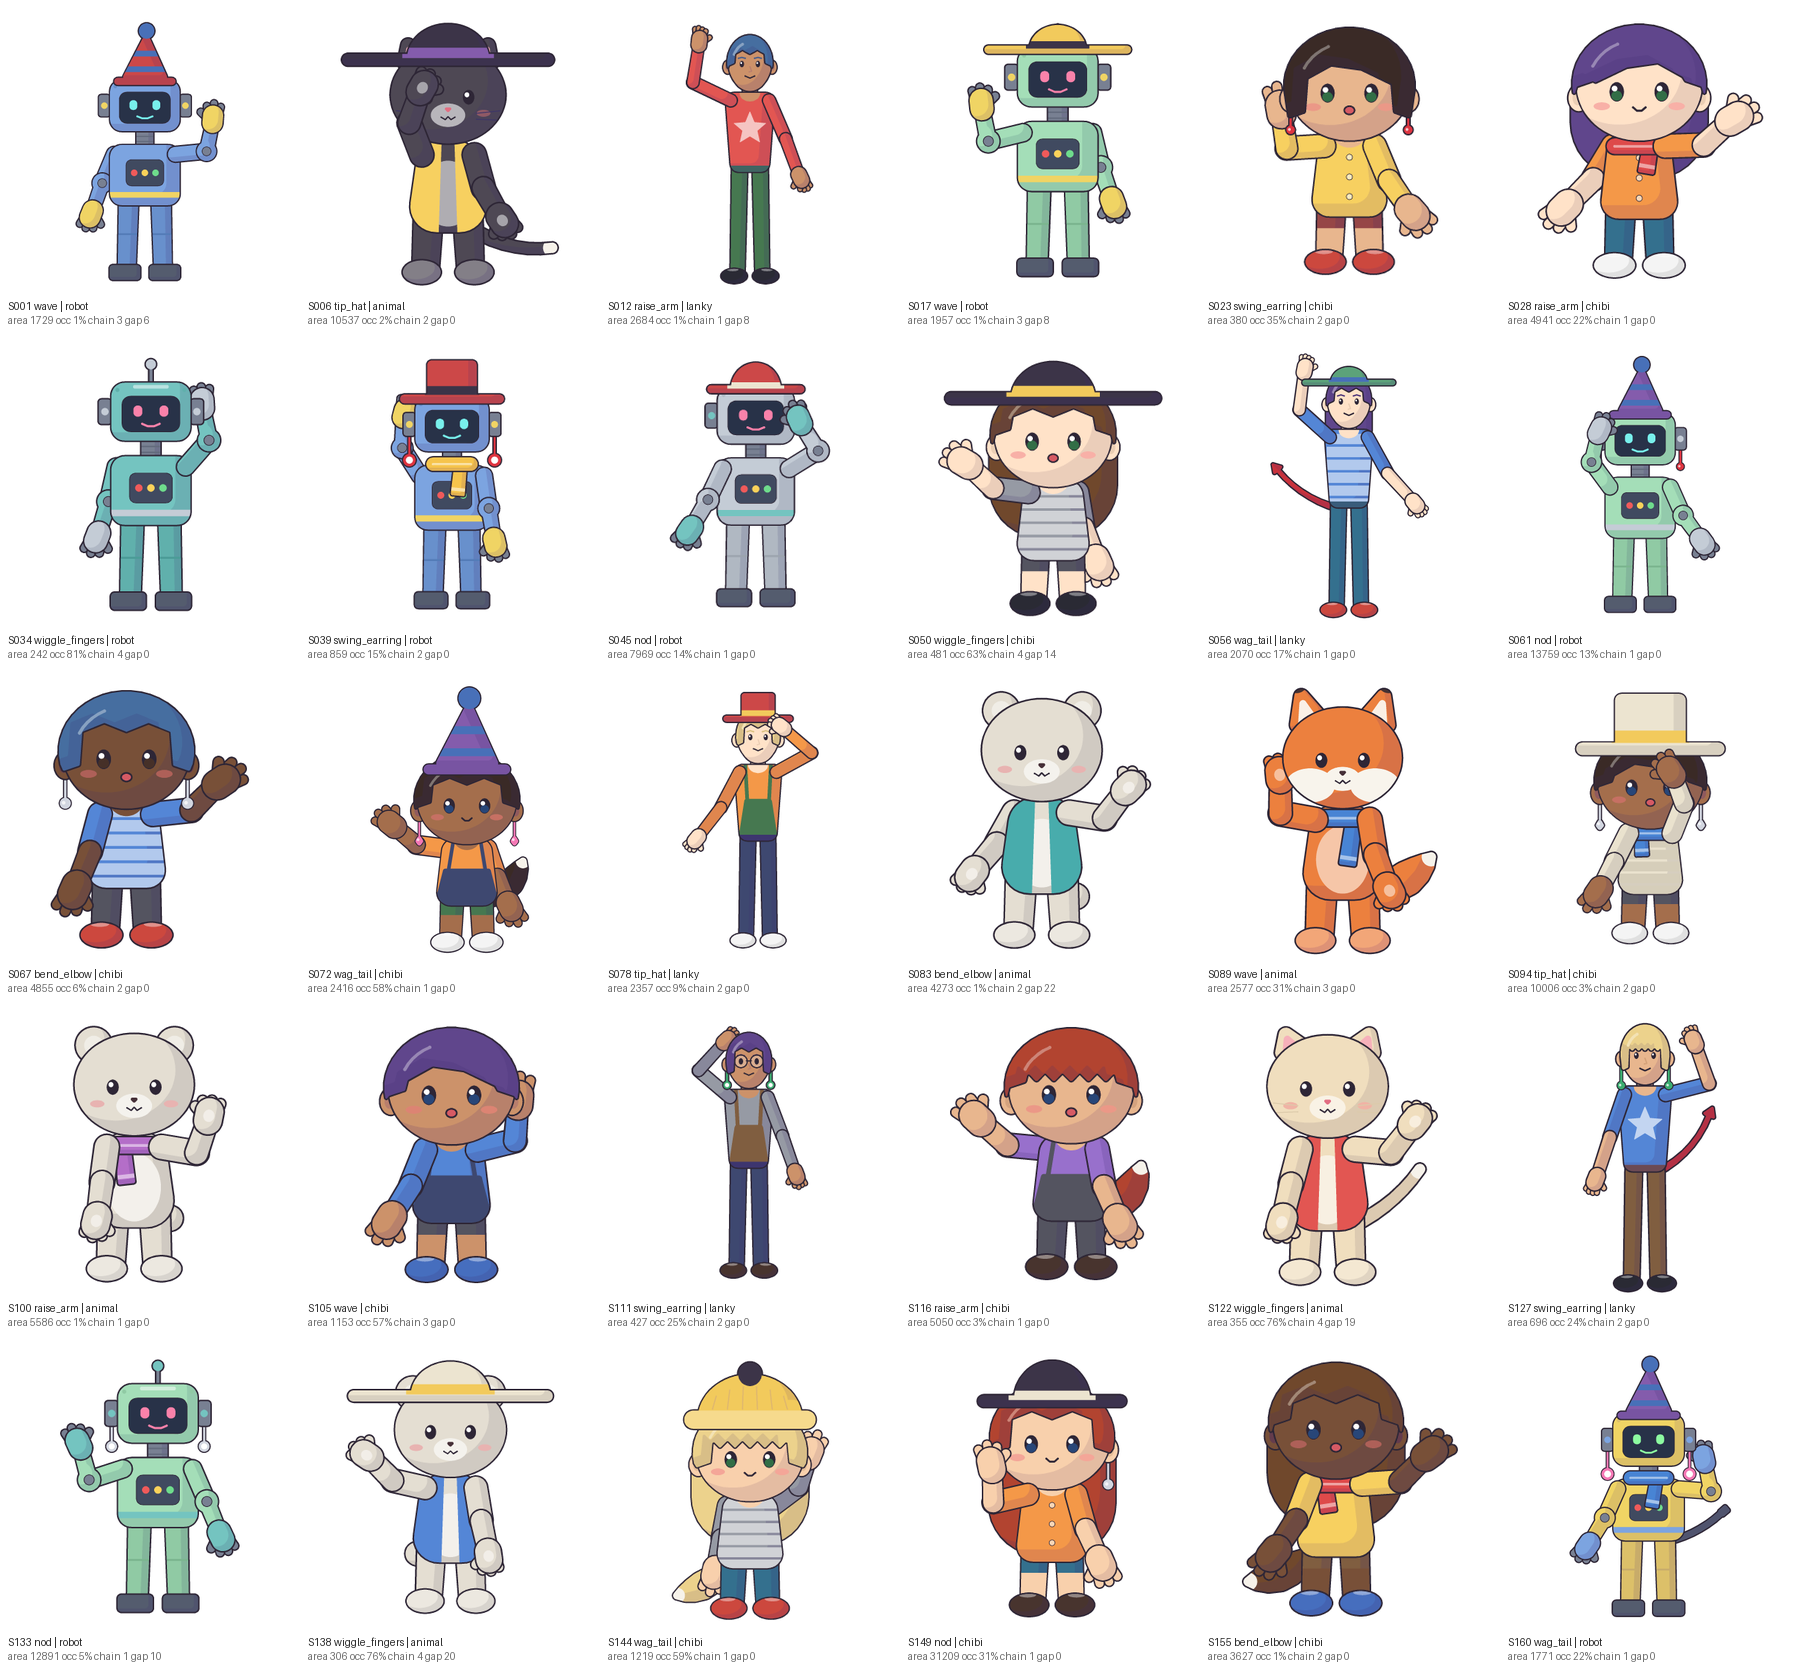
\includegraphics[width=0.82\linewidth]{figs/synth_contact.png}
\caption{Thirty procedural characters, labeled with motion and difficulty factors. Masks and pivots follow from construction, so the procedural split supports controlled analysis of part area, occlusion and chain length.}
\label{fig:synth}
\end{figure}

\section{Evaluation: Separating Change from Side Effects}
\label{sec:checks}

Let $\Delta(a,b)$ be the binary map of pixels whose largest per-channel difference exceeds $\tau=24$, and $\tilde\Delta$ its morphological opening with a $3\times3$ element, which suppresses isolated rendering noise. Let $\phi(x)$ mark foreground pixels, those farther than $30$ from white in some channel. All fractions are maxima over frames.
\begin{align*}
\chk{G1}\ \text{Isolation:}\quad & \max_t \tfrac{|\tilde\Delta(F_t,I)\setminus A^{+}|}{|\overline{A^{+}}|} \le 0.002\\
\chk{G4}\ \text{Motion:}\quad & \max_t \tfrac{|\tilde\Delta(F_t,I)\cap T|}{|T|} \ge 0.20\\
\chk{G5}\ \text{Pivot:}\quad & \max_t \tfrac{|\tilde\Delta(F_t,I)\cap D_{10}(p)\cap T|}{|D_{10}(p)\cap T|} \le 0.30 \quad \forall p\in P \text{ with } |D_{10}(p)\cap T|\ge 30\\
\chk{G6}\ \text{Loop and fidelity:}\quad & \operatorname{mean}\tilde\Delta(F_0,F_{24})\le 0.001 \ \text{ and } \ \operatorname{mean}\tilde\Delta(F_0,I)\le 0.005\\
\chk{G3}\ \text{Area:}\quad & \max_t \tfrac{\max(L_t,\,G_t)}{\max(|\phi(I)\cap T|,\,400)} \le 0.5\\
& \text{and, for hat tasks, } \min_t |\phi(F_t)\cap S| \ge 0.85\,|\phi(I)\cap S|
\end{align*}
where $A^{+}$ is $A$ dilated by $\lceil 0.075\,e(T)\rceil$ pixels, $e(T)$ being the larger side of the part's bounding box, a margin that admits squash and stretch; $D_{10}(p)$ is the disc of radius 10\,px around pivot $p$; and $L_t$ and $G_t$ are the part's area loss and gain in frame $t$, defined below. A pivot that exceeds the \chk{G5} limit still passes if the rigid fit described below is trusted in every offending frame and moves the pivot by at most 4\,px; this rule can only rescue a joint, never fail one. \chk{G2} (Integrity) requires that the number of foreground components of at least 60\,px inside $A$, excluding components whose median contrast against white is below 80, never exceed its value in the source image (or in $F_0$, whichever is larger). \chk{G4}, \chk{G5} and \chk{G6} verify the requested change; \chk{G1}, \chk{G2}, \chk{G2b}, \chk{G2c} and \chk{G3} verify that it causes no side effects.

\paragraph{Connectivity (\chk{G2b}).} \chk{G2} counts components of the whole allowed region, so a thumb left behind that still touches the forearm leaves the count unchanged. \chk{G2b} instead isolates the part in each frame. A foreground pixel inside $A$ is attributed to the part if it lies in the original footprint $T$ (which retains a fragment left behind) or differs from the source by more than $\tau$ (which retains a fragment dragged elsewhere); unchanged pixels outside $T$, such as the parent limb, are excluded, so they cannot reconnect a detached fragment. We count 8-connected pieces of at least 20\,px that retain at least 4\,px after erosion, and fail a frame if it contains more pieces than the source part. Two refinements were each introduced in response to a documented failure of the reference: the raw rather than opened difference map is used, because opening erased thin slivers where the part crossed similar colors (T05, T19); and a piece with no footprint pixel whose border is at least 75\% unchanged scenery is ignored, because a part crossing a similarly colored region produces such enclosed islands (T04, T05, T06, T12, T14).

\paragraph{Rigid fit, residual (\chk{G2c}) and area (\chk{G3}).} \chk{G2b} cannot detect a fragment that remains in contact with the moving part, such as a stationary fingertip swept past by its neighbor. We therefore estimate, in every frame, the rigid pose of each independently moving part by matching edge and texture pixels, with partial credit for pixels that may be hidden behind unchanged scenery; each task ships a label map so that parts are fitted separately. \chk{G2c} fails if a piece of the original part of at least 20\,px remains unchanged (at most 3 per channel) while the fitted motion carries it at least 10\,px away and the moved part does not cover it. The 10\,px threshold was chosen by a sweep from 4 to 12\,px: 4\,px rejected two valid non-rigid bends on T06, while 10\,px retained every detection. The same fit defines \chk{G3}. The loss $L_t$ is the smaller of the fitted loss, which counts pixels behind unchanged scenery as hidden rather than lost, and the drop in the part's own pixel count; the gain $G_t$ is new foreground beyond the part's known occluded area (zero for illustrated tasks). Normalizing by $\max(\text{area}, 400)$ rather than 1000 was necessary to retain detection of the hole corruption on T07, whose earring covers 449\,px.

\paragraph{Admission.} A check is retained for a task only if the reference animation passes it. Of the 21 scored pilot tasks under grader v3, \chk{G2} is dropped on 7, \chk{G5} on 5, \chk{G2c} on 2, and \chk{G2b} on 1 (T19, a lace veil on which connectivity is not meaningful). Table~\ref{tab:thresholds} in the appendix lists all constants.

\paragraph{Statistics.} For model results we report pass@1 estimated from $k$ samples per task and percentile bootstrap intervals over tasks (10{,}000 resamples, seed 0). For validation proportions we report Wilson score intervals.

\section{Validating the Grader}
\label{sec:validate}

\subsection{Detection of seeded corruptions}
\label{sec:detect}

For every scored task we construct up to ten corrupted versions of the reference animation, each designed to violate one property, and record whether any of its intended checks fails. Table~\ref{tab:detect} reports the results for grader v3 alongside v2. Both graders score the same rendered frames, and each receives its own admission.

\begin{table}[t]
\centering
\small
\setlength{\tabcolsep}{4pt}
\begin{tabular}{llrrrc}
\toprule
Corruption & Intended check(s) & v2 & v3 & v3 rate (\%) & v3 95\% CI \\
\midrule
Whole image moves & \chk{G1} & 21/21 & 21/21 & 100.0 & \ci{84.5}{100} \\
Hole left behind & \chk{G3} & 21/21 & 21/21 & 100.0 & \ci{84.5}{100} \\
Frozen part & \chk{G4} & 21/21 & 21/21 & 100.0 & \ci{84.5}{100} \\
Wrong part moves & \chk{G1}/\chk{G4} & 21/21 & 21/21 & 100.0 & \ci{84.5}{100} \\
Centered pivot & \chk{G5} & 12/12 & 16/16 & 100.0 & \ci{80.6}{100} \\
No loop & \chk{G6} & 20/21 & 20/21 & 95.2 & \ci{77.3}{99.2} \\
Detach tip & \chk{G2}/\chk{G2b}/\chk{G2c} & 20/20 & 20/21 & 95.2 & \ci{77.3}{99.2} \\
Gap seam & \chk{G2}/\chk{G2b}/\chk{G2c} & 13/15 & 13/16 & 81.2 & \ci{57.0}{93.4} \\
Detach small & \chk{G2}/\chk{G2b}/\chk{G2c} & 14/20 & 15/21 & 71.4 & \ci{50.0}{86.2} \\
Missed thumb & \chk{G2}/\chk{G2b}/\chk{G2c} & 12/20 & 15/21 & 71.4 & \ci{50.0}{86.2} \\
\midrule
\multicolumn{2}{l}{Corruptions in which the part physically separates} & 57/57 & 57/59 & 96.6 & \ci{88.5}{99.1} \\
\bottomrule
\end{tabular}
\caption{Detection of seeded corruptions on the 21 scored pilot tasks, graders v2 and v3 on identical frames. Denominators count corruptions for which at least one intended check is admitted for the task, and therefore differ between graders.}
\label{tab:detect}
\end{table}

Grader v3 detects more of the detachment families than v2, and every family that does not involve detachment at 95\% or more. Restricted to corruptions in which the part physically separates, verified with an oracle that renders the part alone frame by frame and counts its connected pieces, v3 detects 57 of 59; both misses occur on T19, where the reference fails \chk{G2} and \chk{G2b} on the lace veil, so those checks are dropped, and the flutter rotates by about 6 degrees, too little for the rigid fit. The residual check \chk{G2c} recovers the missed-thumb corruptions that v2 could not detect on T03, T05 and T21, where a stationary fingertip remains in contact with the moving hand, and the detach-small corruption on T03. The remaining misses in the missed-thumb and detach-small families have a different cause: on head tilts (T09 to T11) and jumps (T15, T16), the fragment is left where the moving part covers it, so nothing visible remains behind. We regard this as a limit of any pixel-based test rather than of a particular threshold. For reference, the hackathon grader, which lacked \chk{G2b} and \chk{G2c}, detected 4 of 12 missed-thumb corruptions.

On the procedural split, evaluated on a sample of 64 tasks stratified by motion, v3 detects more detachments than v2 (missed thumb 35 versus 25 of 64; detach small 33 versus 26), but three checks are weak on flat-colored characters in both graders: centered pivot (11 of 64), gap seam (8 of 64) and hole (45 of 64). On flat colors, a rotated joint disc changes almost no pixels, and a vanished part that reveals the exact layers beneath it leaves the pixel count nearly unchanged. The second case cannot arise for a model, which has no access to hidden layers. For the first, the fitted pivot displacement separates the corruptions well: 62 of 65 centered-pivot copies move the fitted pivot by more than 4\,px, against 3 of 65 references. Making this displacement a failing test, not only a rescue, is the principal change planned for the next grader version.

\subsection{Rejection of valid animations}
\label{sec:falsefail}

Detection rates bound only one type of error. A grader tuned against a single reference animation may encode that animation's style and reject valid alternatives, which would penalize capable models. To estimate this error, we implemented 12 animation variants in four families designed to differ from the reference in both motion and implementation: alternative easing and amplitude (sine at three amplitudes, ease-in-out cubic, settling bounce); squash and stretch at two strengths; hierarchical follow-through with two lag values; a two-dimensional canvas renderer and a full-screen shader renderer; and pivots displaced by up to 10\,px. Each variant receives the same inputs as the reference and no grader annotations. Before running them at scale, we wrote down what a human animator would accept for each motion type. We ran all variants on all applicable pilot tasks (242 runs) and classified each failure, with frame-level evidence, as either a valid animation rejected by an overly strict check or a genuine violation by the variant. We report the study for graders v2 and v3, both including \chk{G2b}.

\begin{table}[t]
\centering
\small
\setlength{\tabcolsep}{4pt}
\begin{tabular}{lrrrr}
\toprule
 & \multicolumn{2}{c}{Grader v2} & \multicolumn{2}{c}{Grader v3} \\
\cmidrule(lr){2-3}\cmidrule(lr){4-5}
Check & Applicable & False rejections & Applicable & False rejections \\
\midrule
\chk{G1} Isolation & 242 & 3 & 242 & 0 \\
\chk{G2} Integrity & 136 & 4 & 160 & 0 \\
\chk{G2b} Connectivity & 230 & 27 & 230 & 27 \\
\chk{G2c} Residual & -- & -- & 222 & 0 \\
\chk{G3} Area & 242 & 1 & 242 & 0 \\
\chk{G4} Motion & 242 & 0 & 242 & 0 \\
\chk{G5} Pivot & 144 & 5 & 192 & 7 \\
\chk{G6} Loop & 242 & 0 & 242 & 0 \\
\midrule
Any check (per run) & 242 & 36 (14.9\%) & 242 & 29 (12.0\%) \\
 & & \ci{10.9}{19.9} & & \ci{8.5}{16.7} \\
\bottomrule
\end{tabular}
\caption{False rejections of 242 valid alternative animations (12 variants on up to 21 tasks), with Wilson 95\% intervals for the per-run rate. A failure is a false rejection if no failed check is classified as a genuine violation by the variant.}
\label{tab:falsefail}
\end{table}

Table~\ref{tab:falsefail} summarizes the outcome. We first correct an error in an earlier version of this report, which gave a false-rejection rate of 5.0\%: that analysis omitted \chk{G2b}, which alone falsely rejects 27 valid runs. With \chk{G2b} included, the rate was 14.9\% for grader v2 and is 12.0\% for v3. The changes introduced in v3 remove every false rejection by \chk{G1}, \chk{G2} and \chk{G3}, and the new residual check rejects no valid animation. Motion and loop checks rejected no valid animation under either grader.

The remaining false rejections have two sources. \chk{G2b} accounts for 27: in 20 runs, a valid animation repaints the region uncovered by the moving part in a neighboring color (hair behind the thumb on T02 and T12, hair beneath the lifted hat on T13), and \chk{G2b} counts the repainted region as a loose piece; in 5, white gaps open between strands of the swinging pigtails on T08, which we regard as borderline; and 1 involves pale shirt stripes on T15. Because a left-behind fragment is unchanged by definition, a rule that ignores pieces lying entirely inside the original footprint, containing no unchanged pixel and having a flat color would remove the repaint false alarms without affecting detection; we specify this rule for grader v4 but have not yet re-validated it. \chk{G5} accounts for the other 7 rejections, all under squash and stretch, where deformation moves pixels near the joint.

The study also exposed defects in our own pilot data that a single reference animation could not reveal. The earring mask on T07 excluded the chain, so a bead could separate from its chain without violating any check, and its pivot lay outside the mask, which made \chk{G5} vacuous on that task. The head mask on T10 included a sliver of the raised sleeve. The reference animation on T14 tipped the hat in both directions, contrary to the instruction. Running \chk{G2b} on the alternative animations revealed two further defects: a 402\,px strip of pigtail hair inside a forearm mask (T02, T12) and an 18\,px fleck inside a head mask (T11). All five are corrected in the current task set. We conclude that validating a benchmark against one reference solution is insufficient; independently implemented valid solutions are required at minimum.

\subsection{Grader-induced selection effects}
\label{sec:bias}

The procedural generator screens each candidate configuration by simulating the reference and discarding seeds that fail any check. Of 207 screened seeds, 47 were discarded (22.7\%): 19 by \chk{G3}, 8 by \chk{G2}, 8 because the target was nearly fully hidden, 7 by \chk{G5} and 6 by \chk{G4}. Thirty of the 47 had occlusion enabled. The mechanism is that \chk{G3} treats any change in visible foreground area as damage, while a part that legitimately swings behind another part changes its visible area. Left uncorrected, screening would systematically remove small, occluded parts that move across other parts, which are likely the hardest configurations. This is an instance of a general risk for judge-free benchmarks: when the grader filters the task distribution, its blind spots become the distribution's blind spots. Grader v3 measures area on the part's own pixels and admits \chk{G2b} and \chk{G2c} per task rather than rejecting seeds that fail them. Under v3, 20 seeds are rejected (\chk{G3}: 1), 22 previously rejected configurations are accepted, and the number of tasks with at least 25\% occlusion rises from 65 to 74 of 160 (mean occlusion from 25.2\% to 28.0\%). The reference still passes all 160 tasks in the browser. One consequence is that connectivity is not tested on heavily occluded procedural tasks: \chk{G2b} is dropped on 52 tasks (mean occlusion 44\%, against 20\% where it is kept) and \chk{G2c} on 57.

\section{Preliminary Model Results}
\label{sec:models}

\begin{table}[t]
\centering
\small
\setlength{\tabcolsep}{4pt}
\begin{tabular}{llrrcc}
\toprule
System & Protocol & Tasks & No output & pass@1 (\%) [95\% CI] & Partial (\%) [95\% CI] \\
\midrule
Claude Sonnet 5.5$^\dagger$ & agent & 21 & 0 & 57.1\ci{38.1}{76.2} & 83.5\ci{72.4}{93.0} \\
Kimi K3.1 Pro & single shot & 15 & 0 & 20.0\ci{0.0}{40.0} & 76.5\ci{66.3}{85.8} \\
Qwen 3.8 27B & single shot & 15 & 1 & 20.0\ci{0.0}{40.0} & 68.8\ci{54.2}{81.7} \\
Grok 4.7 & single shot & 14 & 12 & 7.1\ci{0.0}{21.4} & 10.7\ci{0.0}{28.6} \\
DeepSeek V4 Flash Vis. & single shot & 13 & 12 & 7.7\ci{0.0}{23.1} & 7.7\ci{0.0}{23.1} \\
Nemotron 3.5 Super VL & single shot & 21 & 0 & 0.0\ci{0.0}{0.0} & 51.9\ci{46.4}{57.9} \\
Gemini 4 Carbon & single shot & 8 & 8 & 0.0 & 0.0 \\
\bottomrule
\end{tabular}
\caption{Preliminary results from the hackathon runs, one sample per task, re-graded with grader v3 where the generated page was available. $^\dagger$Claude Sonnet 5.5 retains its grades from the hackathon grader, which lacked \chk{G2b} and \chk{G2c}, because its pages were not imported from the evaluation platform; its row is therefore not comparable with the others even in principle. Claude Sonnet 5.5 ran as an agent in Claude Code on Valkyrie; all other systems were queried once through OpenRouter. \emph{No output} counts runs that produced no gradable page, which are scored as failures. Task subsets, protocols and budgets differ across rows, so rows are not comparable.}
\label{tab:models}
\end{table}

Table~\ref{tab:models} reports the only model results currently available. They were collected under a deadline with different protocols, task subsets and token budgets, and we report them to motivate the controlled evaluation, not as findings about model capability. Three observations nevertheless inform its design. First, for three of seven systems, the dominant outcome is the absence of a gradable page (Gemini 8 of 8, DeepSeek 12 of 13, Grok 12 of 14 runs), so their scores measure output budget rather than animation; the controlled evaluation fixes the budget and reports the rate of gradable outputs separately. Second, the re-grade with grader v3 changed 10 of 73 locally rendered runs from pass to fail and none from fail to pass. Kimi K3.1 Pro fell from 9 to 3 of 15 first-attempt passes, Qwen 3.8 27B from 6 to 3 of 15, and Grok 4.7 from 2 to 1 of 14. Eight of the ten are tears detected by \chk{G2b}, including floating fingertips produced by two different systems on the same arm-swing task (T06); two are detected by \chk{G2c} alone, a pinky tip left beside a waving hand (T01) and a strip of veil left beside the arm (T19), both confirmed by inspection. The failure that motivated the benchmark therefore occurs in real model outputs, and the hackathon grader accepted it. Third, for the system with the most complete outputs, Kimi K3.1 Pro, the most frequently failed checks are connectivity (9 of 14 applicable runs), residual (6 of 14), integrity (4 of 10) and pivot (4 of 14), while motion is never failed (0 of 15). With samples of this size the pattern is suggestive only, but it is consistent with the hypothesis that current systems usually produce the requested motion and fail to keep the part whole and correctly localized.

\IfFileExists{sections/cutout.tex}{% Section fragment: included into report.tex via % Section fragment: included into report.tex via % Section fragment: included into report.tex via \input{sections/cutout}.
% Uses only packages and macros defined in report.tex (booktabs, amsmath, natbib,
% \anibench, \chk). Literature snapshot: 17 November 2026. Notes with links and
% dates per claim: docs/research/cutout_notes.md.

\providecommand{\cutrr}{\raggedright}

\section{The Cut-Out Step: Evidence from Prior Work}
\label{sec:cutout}

Inspection of model outputs shows that current systems solve \anibench{} tasks by building a paper cut-out puppet: they estimate an outline polygon for the named part from the image, copy the enclosed pixels into a separate layer, fill the area the layer leaves behind, and rotate the layer about an estimated joint. Each failure we have observed maps onto one step of this procedure. A polygon that is too tight leaves the tip of the part on the background layer (the detached thumb that \chk{G2b} detects); a misplaced joint moves pixels that should stay still (\chk{G5}); a cut line that crosses foreground leaves a seam; and an unfilled or badly filled reveal changes pixels that were never part of the target. Our working hypothesis is that this \emph{cut-out step}, rather than the motion itself, is the capability \anibench{} measures. In the pilot results of Section~\ref{sec:models}, motion (\chk{G4}) is the least frequently failed check, while pivot and integrity checks fail often, which is consistent with the hypothesis but does not test it.

This section reviews what is known about each sub-step for general multimodal models and specifies a diagnostic probe that tests the hypothesis directly. We decompose the cut-out step into four sub-steps: (S1) \emph{localization}, finding the part's pixel extent from its name; (S2) \emph{boundary and thin-part recall}, cutting along the true boundary so that extremities and thin structures are included; (S3) \emph{joint estimation}, placing the pivot; and (S4) \emph{revealed-region fill}, painting what the moved part uncovers. Our main findings are as follows:
\begin{itemize}
\item \textbf{The cut-out step is not solved for parts.} Every class of system that has been evaluated on part-level referring segmentation scores far below its object-level performance. A text-prompted SAM~3 reaches 85.3 gIoU on Pascal objects but 33.1 on PascalPart~\citep{mehrab2026ophrg}, and on GSEval the part subset is the lowest of four subsets for every segmentation model, at 10.0 to 23.1 gIoU~\citep{hu2025groundingsuite}.
\item \textbf{Frontier models find the instance but trace its boundary poorly.} A training-free pipeline in which Gemini emits spline control points as text comes within 5 points of SAM~3 in box AP on LVIS but trails it by 15 points in mask AP~\citep{hamdi2026llmseg}.
\item \textbf{Joint estimation on drawings is unmeasured for general models.} Fine-tuned models that emit keypoints as text match specialist pose estimators on photographs~\citep{wang2024locllm,zhang2025posellm}, but keypoint models transfer poorly to drawings without domain data~\citep{smith2023animateddrawings,chen2022illustratedpose}, and we found no zero-shot evaluation of frontier models on joints.
\item \textbf{Tools help substantially, but a segmenter call does not remove the task.} Iterative zoomed refinement, drawing tools and model-written Python yield gains of 7 to 31 points within the same model~\citep{hamdi2026llmseg,hu2024sketchpad,zhao2025pyvision}, and coupling a planner to SAM~3 gives the best zero-shot reasoning-segmentation results we found~\citep{carion2025sam3}. Yet text-prompted segmenters remain weak on parts, and no tool addresses the pivot or the fill.
\item \textbf{No prior benchmark measures segmentation through an automatically checked action.} The closest precedent is the manually judged ``animation-ready'' rate of Animated Drawings, in which a classical flood-fill pipeline produced usable masks for 42.4\% of drawings and a fine-tuned Mask R-CNN for 24.7\%~\citep{smith2023animateddrawings}.
\end{itemize}

\subsection{Method of This Review}
\label{sec:cutout-method}

A research agent searched arXiv, CVF open access, conference proceedings, the ML Anthology, project pages and developer blogs on 17 November 2026, covering the seven questions listed in \texttt{docs/research/cutout\_notes.md}. Every cited work was opened, and its title, authors, year and venue were copied from the opened page; a venue is given only where that page states one, and the 34 references added in this pass carry the URL of the page that was checked. All numbers below were read from the opened pages (abstracts, HTML full texts or proceedings pages); figures computed by us, such as differences between reported scores, are labeled as such. The page-reading tool returns model-written extracts of long pages, so transcription errors remain possible; we cite only numbers that appeared in tables or abstract text and we did not use values that the tool reconstructed from tables with inferred headers. Several sources were only partly accessible. Per-model PointArena results for Molmo-72B, Gemini-2.5-Pro and Claude appear only in a figure, and removal scores in ImgEdit appear only in a figure; PixelArena and O-Bench report no numbers on their abstract pages; we read the SAM~3 appendix, Bunraku and See-through in parts and may have missed details in the unread portions; dblp blocked automated access; and, as in the positioning memo, social media could not be searched.

\subsection{S1 and S2: Part Extent, Boundaries and Thin Structures}
\label{sec:cutout-seg}

\paragraph{Parts are much harder than objects.} Part-level referring segmentation was introduced as a task with the RefCOCOm benchmark~\citep{wang2024mres}, and three 2025 to 2026 evaluations quantify the gap. On GSEval, a 3{,}800-image benchmark with stuff, part, multi-object and single-object subsets, zero-shot gIoU on parts is 21.2 for LISA-7B, 16.5 for GLaMM and 23.1 for EVF-SAM, against 42.8, 42.1 and 54.5 on single objects~\citep{hu2025groundingsuite}. On InstructPart (2{,}400 images, 44 part classes), object-part queries score between 4.5 (Shikra) and 35.7 (MiniGPT-v2) gIoU, and the authors observe that models ``either obtain the entire object area or miss'' the part~\citep{wan2025instructpart}. GPT-4V, evaluated on a 226-sample subset by grid prompting, reaches 14.1 gIoU, and 25.4 with Set-of-Mark prompting. PARTONOMY reports 5.9\% gIoU for LISA-13B on 862 part labels~\citep{blume2025partonomy}. The gap persists in specialist segmenters: SAM~3 with a text prompt scores 85.3 gIoU on Pascal objects, 33.1 on PascalPart, 53.9 on PartImageNet and 71.1 on InstructPart~\citep{mehrab2026ophrg}. These results are consistent across benchmarks, but none of them evaluates the current frontier API models on parts with a pixel metric.

\paragraph{Geometry emitted as text.} An \anibench{} agent without tools must express a part's extent as coordinates in code, so models that output geometry as text are the relevant comparison. PolyFormer generates polygon vertices autoregressively and regresses floating-point coordinates to avoid quantization error~\citep{liu2023polyformer}. Text4Seg instead labels image patches with text and finds a $16\times16$ grid competitive~\citep{lan2025text4seg}; on a 1200$\times$600 pilot image, each cell of such a grid covers about 2{,}800\,px, comparable to an entire hand in our pilot tasks (2{,}301 to 5{,}294\,px). The most informative result is LLMSeg, in which an off-the-shelf Gemini model detects a box, emits closed B-spline or polygon loops as JSON in absolute pixel coordinates, and refines them around residual errors~\citep{hamdi2026llmseg}. It reaches 71.5 cIoU on ReasonSeg validation without segmentation training. Two of its results bear directly on \anibench{}. First, refinement accounts for much of the quality: removing it lowers ReasonSeg cIoU from 74.7 to 67.2 and RefCOCO cIoU from 79.8 to 64.6, at the cost of 14.6 rather than 2.0 model calls per item. Second, on matched LVIS items its box AP approaches that of SAM~3 (64.2 against 69.1) while its mask AP does not (47.2 against 62.2; on COCO, 50.5 against 59.2), and the author lists imprecise pixel-level boundaries as a limitation. Forcing straight-edged polygons instead of splines changes ReasonSeg cIoU by less than the run-to-run standard deviation (73.1 against 74.7). A separate evaluation that drives API models through prompt chains finds the same ordering: on COCO semantic segmentation through superpixels, GPT-4o reaches 44.9 mIoU, Gemini 2.0 Flash 43.0 and Claude 3.5 Sonnet 32.1, against 65.5 for a specialist, and models perform better on semantic than on geometric tasks~\citep{ramachandran2025gpt4ovision}. Marking regions directly on the full image, without crops, lowers GPT-4o's result to 25.8 mIoU in that study's ablation.

\paragraph{Thin structures and boundaries.} Thin, elongated structures are a known failure of segmenters in general. Interactive segmenters often fail on parts such as insect legs because thin pixels are rare and imbalanced against the rest of the object, which motivated the ThinObject-5K dataset and an IoU computed on thin regions only~\citep{liew2021thinobject}; SAM's masks degrade on objects with intricate structure~\citep{ke2023hqsam}. Standard mask IoU hides these errors on larger parts, because interior area grows quadratically with size while the contour grows linearly~\citep{cheng2021boundaryiou}. We found no paper that reports a boundary or thin-structure metric for part segmentation by multimodal language models. This is an absence of evidence rather than evidence of competence.

\subsection{S1 and S3: Coordinates and Joints}
\label{sec:cutout-coords}

\paragraph{Pointing and coordinate precision.} On Point-Bench, where a point counts as correct if it falls inside the target mask, GPT-4o averages 29.5\% and Gemini-2.5-Flash 46.8\%; Molmo-72B and Gemini-2.5-Pro are statistically indistinguishable at the top~\citep{cheng2025pointarena}. Explicit pointing supervision is the largest factor: models trained without it score 4.8 to 17.4\%, while a 7B model trained with pointing data reaches 52.3\%, against 17.4\% for its predecessor without such data~\citep{cheng2025pointarena,deitke2025molmo}. Precision degrades with resolution and target size. On high-resolution professional screenshots with small targets, the best existing grounding model reaches 18.9\%, and a planner-guided search that progressively narrows the region reaches 48.1\% without training~\citep{li2025screenspotpro}. Accuracy falls when the relevant detail is small, although the model's attention still lands on it, so cropping guided by that attention recovers much of the loss~\citep{zhang2025wheretolook}. Coordinate errors at high resolution are directional rather than random, which one study attributes to degraded positional encodings~\citep{tao2025coordbias}. On simple geometric judgments, such as whether two circles overlap, four models that were state of the art in 2024 averaged 58.1\%~\citep{rahmanzadehgervi2024blind}.

\paragraph{Joints.} Language models can emit keypoints as text with specialist accuracy once fine-tuned: on COCO with ground-truth boxes, PoseLLM reaches 77.8 AP and LocLLM 77.4, equal to or above the heatmap model ViTPose at 77.4~\citep{zhang2025posellm,wang2024locllm}, and category-agnostic variants exist~\citep{kim2025capellm}. Drawings are a different domain. A COCO-pretrained keypoint model scores 0.696 PCKh@50 on illustrated characters, and transfer learning with 4{,}000 annotated illustrations raises it to 0.787~\citep{chen2022illustratedpose}; on children's drawings, a pose model reaches 0.09 mAP before fine-tuning and 0.85 to 0.90 after~\citep{smith2023animateddrawings}. We found no evaluation of frontier general-purpose models on zero-shot joint localization in either domain. The pivot an \anibench{} task requires is also not a keypoint in the pose-estimation sense: it lies on the interface between the part and its parent (for example the wrist line), so a model can name the correct joint and still misplace the rotation center by more than the 10\,px radius that \chk{G5} tolerates.

\subsection{Tool Use}
\label{sec:cutout-tools}

Coupling a language model to a segmenter is the most effective route to referring segmentation that we found. In SAM~3 Agent, a multimodal model calls SAM~3 with noun phrases, inspects the returned masks and selects among them; with Gemini 2.5 Pro as the planner it reaches 74.0 gIoU on the ReasonSeg test split, against 57.5 for Seg-Zero, which trains a 7B model to emit prompts for a frozen segmenter~\citep{carion2025sam3,liu2025segzero}. The SAM~3 appendix does not report the same planners without the tool, so the gain attributable to the tool itself is not isolated. SegAgent trains a model to emit click points for an interactive segmenter over several steps~\citep{zhu2025segagent}. Generic visual tools also help: drawing with detection and segmentation tools improves vision tasks by 8.6 points on average~\citep{hu2024sketchpad}; code generation against a vision API needs no training~\citep{suris2023vipergpt}; and letting the model write and run its own Python tools improves Claude-4.0-Sonnet by 31.1 points on VLMsAreBlind-mini~\citep{zhao2025pyvision}.

Two qualifications matter for \anibench{}. First, a text-prompted segmenter does not resolve parts: the SAM~3 result on PascalPart (33.1 gIoU) shows that ``segment the thumb'' is not a solved call. A point-prompted segmenter would change this, because it reduces extent estimation to pointing at the part, which Point-Bench measures. Second, classical image-processing code is a credible alternative on line art. Animated Drawings segments characters with adaptive thresholding, morphological closing and flood fill, and this pipeline produced animation-ready masks for 42.4\% of 571 drawings, against 24.7\% for a Mask R-CNN fine-tuned on 2{,}500 drawings~\citep{smith2023animateddrawings}. Its failures, which include separately drawn body parts, limbs that touch at non-joint points and outlines that are not closed, are the cases in which a flood fill crosses into a neighbor or stops short of a tip. We found no study of a language-model agent writing such code for a named part.

\subsection{S4: Layers, Amodal Completion and the Revealed Region}
\label{sec:cutout-fill}

Generative methods now decompose a single illustration into layers with the occluded content completed. See-through produces 19 inpainted RGBA layers per anime character and improves on a segment-then-inpaint baseline (SAM with LaMa) from 0.288 to 0.155 LPIPS~\citep{lin2026seethrough,suvorov2022lama}. Bunraku fine-tunes a layered diffusion model~\citep{yin2025qwenimagelayered} on 10{,}000 Live2D models with a loss on occluded regions and adds per-layer meshes and deformation offsets~\citep{chen2026bunraku}. Earlier work generates transparent layers directly~\citep{zhang2024layerdiffuse} and completes occluded objects zero-shot, including in artwork~\citep{ozguroglu2024pix2gestalt,ao2025amodal}. For general models the evidence is weaker: 22 multimodal models fall significantly short of humans on occlusion perception, and neither scale nor reasoning closes the gap~\citep{liu2025obench}; instruction-based editors can remove objects, but their errors include blurred results, removal of adjacent objects and changes to unrelated regions~\citep{ye2025imgedit,qian2025giebench}. None of these works asks a code-writing model to fill a revealed region, and none reports joint or pivot error. When a part moves over white background, S4 reduces to painting white; it becomes difficult when the part lies over other foreground, which describes the occluded configurations that the area check disproportionately removed during procedural screening (Section~\ref{sec:bias}).

\subsection{Prior Cut-Out Animation Systems and How They Evaluate}
\label{sec:cutout-puppet}

Cut-out animation from one image has a standard pipeline: segment the character, place joints, and deform the image with a skeleton or with handle-driven as-rigid-as-possible deformation of a triangle mesh~\citep{igarashi2005arap}. Animated Drawings is the most completely evaluated instance~\citep{smith2023animateddrawings}. It reports detection, segmentation and pose accuracy separately, and also the rate at which each stage yields an animation-ready result by visual inspection: 90.2\% for pose, 42.4\% for classical segmentation, and 39.4\% for the full pipeline. Users corrected 20\% of masks in a 5{,}000-image sample of the released data. Systems that animate articulated objects with model-written code evaluate joint parameters through the simulated result, not through a coordinate error~\citep{le2025articulateanything}. Layer-decomposition systems evaluate image similarity of the layers and the quality of deformations, not segmentation boundaries or pivots~\citep{lin2026seethrough,chen2026bunraku}. Table~\ref{tab:cutout-works} summarizes the comparison.

\begin{table}[t]
\centering
\footnotesize
\setlength{\tabcolsep}{3pt}
\begin{tabular}{@{}p{2.9cm}p{2.2cm}p{1.3cm}p{2.3cm}p{1.4cm}p{1.2cm}p{2.6cm}@{}}
\toprule
\cutrr Work & \cutrr Output form & \cutrr Part-level & \cutrr Boundary or thin metric & \cutrr Joint & \cutrr Fill & \cutrr Scored through action \tabularnewline
\midrule
\cutrr GSEval~\citep{hu2025groundingsuite} & \cutrr mask & \cutrr yes & \cutrr no & \cutrr no & \cutrr no & \cutrr no \tabularnewline
\cutrr InstructPart~\citep{wan2025instructpart} & \cutrr mask & \cutrr yes & \cutrr no & \cutrr no & \cutrr no & \cutrr no (affordance queries) \tabularnewline
\cutrr OP-HRG~\citep{mehrab2026ophrg} & \cutrr box, points, mask & \cutrr yes & \cutrr no & \cutrr no & \cutrr no & \cutrr no \tabularnewline
\cutrr LLMSeg~\citep{hamdi2026llmseg} & \cutrr splines as text & \cutrr no & \cutrr no & \cutrr no & \cutrr no & \cutrr no \tabularnewline
\cutrr SAM~3 Agent~\citep{carion2025sam3} & \cutrr tool calls & \cutrr no & \cutrr no & \cutrr no & \cutrr no & \cutrr no \tabularnewline
\cutrr Point-Bench~\citep{cheng2025pointarena} & \cutrr point as text & \cutrr partly & \cutrr no & \cutrr no & \cutrr no & \cutrr robot use, user-rated \tabularnewline
\cutrr LocLLM, PoseLLM~\citep{wang2024locllm,zhang2025posellm} & \cutrr keypoints as text & \cutrr n/a & \cutrr no & \cutrr yes (PCK, AP) & \cutrr no & \cutrr no \tabularnewline
\cutrr Animated Drawings~\citep{smith2023animateddrawings} & \cutrr mask, keypoints & \cutrr no & \cutrr no & \cutrr yes (AP) & \cutrr no & \cutrr yes, by inspection \tabularnewline
\cutrr See-through~\citep{lin2026seethrough} & \cutrr RGBA layers & \cutrr yes & \cutrr no & \cutrr no & \cutrr yes (image metrics) & \cutrr no \tabularnewline
\cutrr Bunraku~\citep{chen2026bunraku} & \cutrr layers, meshes & \cutrr yes & \cutrr no & \cutrr no & \cutrr loss only & \cutrr animation, vertex cosine \tabularnewline
\midrule
\cutrr \anibench{} & \cutrr three.js program & \cutrr yes & \cutrr via \chk{G2b} & \cutrr via \chk{G5} & \cutrr via \chk{G1}, \chk{G3} & \cutrr yes, deterministic \tabularnewline
\cutrr \anibench{} probe (proposed) & \cutrr polygon, mask, pivot & \cutrr yes & \cutrr yes & \cutrr yes & \cutrr yes (procedural) & \cutrr linked to checks \tabularnewline
\bottomrule
\end{tabular}
\caption{Prior work on the sub-steps of the cut-out, by what it outputs and measures. ``Fill'' refers to completion of a region revealed or occluded by a part. ``Scored through action'' indicates that segmentation or localization is evaluated by the success of a downstream use.}
\label{tab:cutout-works}
\end{table}

\subsection{Measuring Cut-Out Quality Directly}
\label{sec:cutout-metrics}

Four families of metrics apply. \emph{Region overlap} (mask IoU) is standard but insensitive to boundary error on large parts. \emph{Boundary metrics} restrict scoring to a band around the contour: Boundary IoU computes IoU over mask pixels within distance $d$ of either contour, with a default of 2\% of the image diagonal~\citep{cheng2021boundaryiou}, and the contour accuracy of DAVIS matches boundary pixels within a tolerance~\citep{perazzi2016davis}. The default $d$ corresponds to about 27\,px on our 1200$\times$600 pilot images, which exceeds the radius of every pilot hand, so a fixed small band is needed. \emph{Thin-structure metrics} score thin regions separately, as with IoU on thin regions~\citep{liew2021thinobject}, or compare skeletons to guarantee topology preservation, as with clDice~\citep{shit2021cldice}. \emph{Joint metrics} use distances normalized by part or body size, as in PCK. Our own measurements on the 24 pilot target masks show why thin-structure metrics alone are insufficient for \anibench{}: the fraction of target pixels removed by a $7\times7$ morphological opening, which approximates the fraction in structures narrower than 7\,px, has a median of 0.5\% and ranges from 1.4\% to 3.1\% for hands, reaching 13.3\% only for the earrings of T07. The detached thumb is therefore a failure at an \emph{extremity}, far from the joint, rather than in a sub-7-px structure, and the probe below adds a metric for extremities.

\subsection{A Diagnostic Probe for \anibench{}}
\label{sec:cutout-probe}

The probe asks each model to perform the cut-out explicitly, scores the result against our ground-truth masks and pivots, and relates the scores to the same model's animation outcomes on the same task. Correlation alone cannot establish that cut-out errors cause animation failures, so the probe also substitutes ground truth for each sub-step and measures the change in pass rate.

\paragraph{Arms.} Each arm runs in a fresh session with the same image bytes and instruction as the animation task and never sees grader annotations.
\begin{itemize}
\item \textbf{P0, explicit without tools.} One response in JSON of the form
\[\texttt{\{"polygons": [[[x,y],\dots]], "holes": [\dots], "pivots": [[x,y],\dots]\}}\]
in pixel coordinates of the original image, whose width and height are stated in the prompt. We rasterize with even-odd filling at the original resolution.
\item \textbf{P1, explicit with code.} The agent may run Python with NumPy, SciPy, Pillow and OpenCV but no pretrained models, and writes \texttt{mask.png}, \texttt{pivot.json} and \texttt{plate.png}, the image with the part removed and the uncovered region filled.
\item \textbf{P2, explicit with a segmenter.} As P1, with a point-, box- and text-promptable SAM-family tool. This arm estimates how much of the cut-out a segmenter supplies.
\item \textbf{I, implicit.} No new model call. From the frames of the model's own animation run, we compute the extremity residue defined below, which estimates how much of the part's tip was left behind, without parsing the code.
\end{itemize}

\paragraph{Metrics.} Let $T$ be the ground-truth target mask, $\hat M$ the predicted mask, $p^\ast$ the ground-truth pivot and $\hat p$ the predicted one, $\phi$ the foreground map of Section~\ref{sec:checks}, and $\Delta$ the raw change map with $\tau=24$.
\begin{itemize}
\item \emph{Extent:} $\mathrm{IoU}(\hat M,T)$ and Boundary IoU with a fixed band $d=3$\,px, reported together with $d$ equal to 5\% of the diagonal of $T$'s bounding box.
\item \emph{Extremity recall:} let $g(x)$ be the geodesic distance within $T$ from $x$ to the nearest pivot, and $E=\{x\in T: g(x)\ge q_{0.9}(g)\}$ the 10\% of the part farthest from its joint. Then $R_{\mathrm{ext}}=|\hat M\cap E|/|E|$. Defined for tasks with at least one pivot.
\item \emph{Thin recall:} $T_{\mathrm{thin}}=T\setminus \mathrm{open}(T,7\times7)$ and $R_{\mathrm{thin}}=|\hat M\cap T_{\mathrm{thin}}|/|T_{\mathrm{thin}}|$, reported only where $|T_{\mathrm{thin}}|\ge 20$\,px.
\item \emph{Predicted residue:} the number of pieces of $T\setminus\hat M$ that would count under \chk{G2b} (at least 20\,px, at least 4\,px after a $3\times3$ erosion). A positive count predicts a left-behind fragment.
\item \emph{Leakage:} $L_{\mathrm{fg}}=|(\hat M\setminus T)\cap\phi(I)|/|T|$, foreground of other parts that would be torn away, and $L_{\mathrm{bg}}=|(\hat M\setminus T)\setminus\phi(I)|/|T|$, background that would be carried over neighbors.
\item \emph{Pivot error:} $e=\lVert\hat p-p^\ast\rVert_2$ in pixels, with a hit if $e\le 10$\,px (the \chk{G5} radius), and $e/\sqrt{|T|}$ with PCK at 0.1 and 0.2. Multiple pivots are matched by minimum-cost assignment.
\item \emph{Fill error} (procedural split only, where the generator provides the true plate $P$): the fraction of pixels in $T$ for which the submitted plate differs from $P$ by more than $\tau$ in some channel, reported separately for pixels where $P$ is background and where $P$ is foreground.
\item \emph{Extremity residue} (arm I): $\rho=|E\cap\bigcap_t \neg\Delta(F_t,I)|/|E|$, the fraction of the extremity that never changes in any frame. Under a rotation about the true joint, extremity pixels move the farthest, so an unchanged extremity pixel indicates a fragment left behind, unless it lies over a neighbor of the same color, which we flag using the \chk{G2b} scenery test.
\end{itemize}

\paragraph{Analyses.} (1) \emph{Profiles:} the distribution of each metric by model and arm, stratified by part-area tercile. (2) \emph{Prediction:} for each run, we test whether the predicted residue predicts \chk{G2b} failure, pivot error predicts \chk{G5} failure, and leakage predicts \chk{G1} failure, reporting AUROC with percentile bootstrap intervals clustered by source image, and logistic regressions with model fixed effects and the recorded difficulty factors (area, occlusion, chain length). On the 160-task procedural split with a 30\% failure rate, an AUROC of 0.7 has a 95\% interval of roughly $\pm0.09$ (our calculation, Hanley and McNeil approximation), adequate to distinguish predictive from uninformative metrics. (3) \emph{Agreement between arms:} the correlation between $R_{\mathrm{ext}}$ in P0 and $1-\rho$ in arm I tests whether the explicit probe reflects what the model does when animating. (4) \emph{Oracle substitution:} we re-run the animation task with the ground-truth mask (as an alpha matte file), the ground-truth pivot, both, and on the procedural split both plus the true plate. The increase in pass rate under each substitution attributes failures to sub-steps.

\paragraph{Decision rule.} We will regard the hypothesis as supported if (i) supplying the mask and pivot converts at least half of the failing runs into passes and (ii) at least one probe metric predicts its corresponding check with an AUROC interval above 0.5. If substitution recovers few failures, the bottleneck lies in motion synthesis or program execution, and the paper should not describe \anibench{} as a cut-out benchmark.

\paragraph{Confounds and controls.} \emph{Coordinate conventions:} some models natively emit coordinates on a 0 to 1000 grid~\citep{hamdi2026llmseg}; we pilot three formats (absolute pixels, normalized to $[0,1]$, 0 to 1000) on five held-out images and fix each model's best format before scoring. \emph{Resizing:} APIs may downsample the image; we record the resolution each model receives and add a tiled-crop condition on a subset, because crops change localization accuracy~\citep{li2025screenspotpro,zhang2025wheretolook}. \emph{Annotation ambiguity:} where the hand ends at the wrist, and where the pivot lies, are matters of judgment; a second author annotates 30 parts independently, and we report human-to-human IoU, Boundary IoU and pivot error as a ceiling. The defective T07 and T10 masks are corrected first (Section~\ref{sec:falsefail}). \emph{Mechanical coupling:} \chk{G2b} and the residue metric use the same $T$, and \chk{G5} responds to cut lines near the joint as well as to pivot error, so some correlation is expected by construction; causal statements rest on substitution, not on correlation. \emph{Session effects:} probe and animation runs are separate sessions with randomized order. \emph{Size:} extremity and thin metrics covary with part area, hence the stratification.

\subsection{Synthesis and Implications}
\label{sec:cutout-synthesis}

\paragraph{Status of each sub-step.} Table~\ref{tab:cutout-steps} summarizes the evidence. Locating the object that contains a part is close to solved for frontier models at the box level. Recovering the part's extent is not solved for any class of system, and its boundary is the weakest measured component: the gap between box and mask accuracy, and the gains from iterative zoomed refinement, both indicate that models know approximately where the part is but not exactly where it ends. Joint estimation on drawings and revealed-region fill are not measured for general models, so the literature cannot rank them; the pilot's frequent \chk{G5} failures suggest that joint estimation may be as weak as boundary recall. The probe is designed to separate these possibilities.

\begin{table}[t]
\centering
\footnotesize
\setlength{\tabcolsep}{3pt}
\begin{tabular}{@{}p{2.5cm}p{6.0cm}p{3.0cm}p{2.4cm}@{}}
\toprule
\cutrr Sub-step & \cutrr Strongest evidence & \cutrr Measured for frontier general models? & \cutrr Assessment \tabularnewline
\midrule
\cutrr S1 instance localization & \cutrr LLMSeg box AP 64.2 vs.\ SAM~3 69.1; Point-Bench 29.5 to 46.8\% & \cutrr yes & \cutrr largely solved for objects \tabularnewline
\cutrr S1 part extent & \cutrr PascalPart 33.1 gIoU (SAM~3); GSEval part 10.0 to 23.1 gIoU; InstructPart 4.5 to 35.7 & \cutrr no (GPT-4V subset only) & \cutrr unsolved \tabularnewline
\cutrr S2 boundary and extremities & \cutrr LLMSeg mask AP 47.2 vs.\ 62.2; refinement +7.5 to +15.2 cIoU; thin-object failures in specialists & \cutrr partly (mask AP) & \cutrr weakest measured \tabularnewline
\cutrr S3 joint (pivot) & \cutrr fine-tuned text keypoints 77.8 AP on photos; drawings 0.09 mAP untuned & \cutrr no & \cutrr unmeasured risk \tabularnewline
\cutrr S4 revealed fill & \cutrr generative layer decomposition; MLLM occlusion perception below humans & \cutrr no & \cutrr unmeasured \tabularnewline
\bottomrule
\end{tabular}
\caption{Evidence on each sub-step of the cut-out. Numbers are from the works cited in Sections~\ref{sec:cutout-seg} to \ref{sec:cutout-fill}.}
\label{tab:cutout-steps}
\end{table}

\paragraph{Framing.} The evidence supports describing \anibench{} as a test of part-level grounding, joint inference and reveal handling \emph{measured through an action whose consequences are checked deterministically}. No benchmark we found does this, and the closest precedent relies on manual inspection~\citep{smith2023animateddrawings}. The framing also answers a likely objection, that \anibench{} is part segmentation with extra steps: a static segmentation benchmark scores a mask, whereas \anibench{} scores whether the mask, the pivot and the fill together yield a correct motion, and the probe shows how much each contributes. We recommend against describing the benchmark as a test of general ``spatial understanding'' until the probe has been run.

\paragraph{Task design.} The pilot under-samples the structures on which segmentation is known to fail. We recommend adding parts with thin or protruding structure (spread fingers, tails, antennae, chains, whiskers), parts that move across other foreground so that the cut line and the fill both matter, and parts adjacent to similarly colored neighbors. The last category requires care, because \chk{G2b} ignores islands enclosed by same-colored scenery (Section~\ref{sec:checks}). Each task should record three further difficulty factors: thin fraction, extremity distance relative to part size, and the fraction of the reveal that lies over foreground. The selection effect of Section~\ref{sec:bias} matters here, because it disproportionately removed occluded configurations, in which S4 is hard.

\paragraph{Settings.} If a segmenter call solved the task, \anibench{} would measure tool orchestration rather than perception. The evidence indicates that it does not: text-prompted segmenters are weak on parts, a point-prompted segmenter still requires the model to localize the part, and no segmenter supplies the pivot or the fill. We therefore recommend three tool tiers, reported separately: no code execution beyond the page; general code without pretrained vision models, which permits thresholds and flood fills that are legitimate on line art; and code with a segmenter. The difference between tiers is itself a finding, and each run should be labeled by the strategy it used (estimated polygon, color-based or flood-fill selection, segmenter), which can be read from the transcript.

\paragraph{Limitations.} This review covers the literature, not our models: every statement about \anibench{} failures remains a hypothesis until the probe is run. The part-segmentation evidence comes mostly from photographs and from models older than the systems in Table~\ref{tab:models}; frontier models of late 2026 have not been evaluated on part-level masks in any work we found, and the cartoon domain may be easier, because outlines and flat colors favor both segmentation and flood fills, or harder, because pretrained models see fewer drawings. Several comparisons above, such as object against part performance, combine scores from different benchmarks and indicate a direction rather than a magnitude. Our pilot measurements of thin structure use 24 masks from two illustrations. Finally, the probe's explicit arms may not reflect what a model does when it writes animation code; arm I and the agreement analysis are included to detect this, but cannot exclude it.
.
% Uses only packages and macros defined in report.tex (booktabs, amsmath, natbib,
% \anibench, \chk). Literature snapshot: 17 November 2026. Notes with links and
% dates per claim: docs/research/cutout_notes.md.

\providecommand{\cutrr}{\raggedright}

\section{The Cut-Out Step: Evidence from Prior Work}
\label{sec:cutout}

Inspection of model outputs shows that current systems solve \anibench{} tasks by building a paper cut-out puppet: they estimate an outline polygon for the named part from the image, copy the enclosed pixels into a separate layer, fill the area the layer leaves behind, and rotate the layer about an estimated joint. Each failure we have observed maps onto one step of this procedure. A polygon that is too tight leaves the tip of the part on the background layer (the detached thumb that \chk{G2b} detects); a misplaced joint moves pixels that should stay still (\chk{G5}); a cut line that crosses foreground leaves a seam; and an unfilled or badly filled reveal changes pixels that were never part of the target. Our working hypothesis is that this \emph{cut-out step}, rather than the motion itself, is the capability \anibench{} measures. In the pilot results of Section~\ref{sec:models}, motion (\chk{G4}) is the least frequently failed check, while pivot and integrity checks fail often, which is consistent with the hypothesis but does not test it.

This section reviews what is known about each sub-step for general multimodal models and specifies a diagnostic probe that tests the hypothesis directly. We decompose the cut-out step into four sub-steps: (S1) \emph{localization}, finding the part's pixel extent from its name; (S2) \emph{boundary and thin-part recall}, cutting along the true boundary so that extremities and thin structures are included; (S3) \emph{joint estimation}, placing the pivot; and (S4) \emph{revealed-region fill}, painting what the moved part uncovers. Our main findings are as follows:
\begin{itemize}
\item \textbf{The cut-out step is not solved for parts.} Every class of system that has been evaluated on part-level referring segmentation scores far below its object-level performance. A text-prompted SAM~3 reaches 85.3 gIoU on Pascal objects but 33.1 on PascalPart~\citep{mehrab2026ophrg}, and on GSEval the part subset is the lowest of four subsets for every segmentation model, at 10.0 to 23.1 gIoU~\citep{hu2025groundingsuite}.
\item \textbf{Frontier models find the instance but trace its boundary poorly.} A training-free pipeline in which Gemini emits spline control points as text comes within 5 points of SAM~3 in box AP on LVIS but trails it by 15 points in mask AP~\citep{hamdi2026llmseg}.
\item \textbf{Joint estimation on drawings is unmeasured for general models.} Fine-tuned models that emit keypoints as text match specialist pose estimators on photographs~\citep{wang2024locllm,zhang2025posellm}, but keypoint models transfer poorly to drawings without domain data~\citep{smith2023animateddrawings,chen2022illustratedpose}, and we found no zero-shot evaluation of frontier models on joints.
\item \textbf{Tools help substantially, but a segmenter call does not remove the task.} Iterative zoomed refinement, drawing tools and model-written Python yield gains of 7 to 31 points within the same model~\citep{hamdi2026llmseg,hu2024sketchpad,zhao2025pyvision}, and coupling a planner to SAM~3 gives the best zero-shot reasoning-segmentation results we found~\citep{carion2025sam3}. Yet text-prompted segmenters remain weak on parts, and no tool addresses the pivot or the fill.
\item \textbf{No prior benchmark measures segmentation through an automatically checked action.} The closest precedent is the manually judged ``animation-ready'' rate of Animated Drawings, in which a classical flood-fill pipeline produced usable masks for 42.4\% of drawings and a fine-tuned Mask R-CNN for 24.7\%~\citep{smith2023animateddrawings}.
\end{itemize}

\subsection{Method of This Review}
\label{sec:cutout-method}

A research agent searched arXiv, CVF open access, conference proceedings, the ML Anthology, project pages and developer blogs on 17 November 2026, covering the seven questions listed in \texttt{docs/research/cutout\_notes.md}. Every cited work was opened, and its title, authors, year and venue were copied from the opened page; a venue is given only where that page states one, and the 34 references added in this pass carry the URL of the page that was checked. All numbers below were read from the opened pages (abstracts, HTML full texts or proceedings pages); figures computed by us, such as differences between reported scores, are labeled as such. The page-reading tool returns model-written extracts of long pages, so transcription errors remain possible; we cite only numbers that appeared in tables or abstract text and we did not use values that the tool reconstructed from tables with inferred headers. Several sources were only partly accessible. Per-model PointArena results for Molmo-72B, Gemini-2.5-Pro and Claude appear only in a figure, and removal scores in ImgEdit appear only in a figure; PixelArena and O-Bench report no numbers on their abstract pages; we read the SAM~3 appendix, Bunraku and See-through in parts and may have missed details in the unread portions; dblp blocked automated access; and, as in the positioning memo, social media could not be searched.

\subsection{S1 and S2: Part Extent, Boundaries and Thin Structures}
\label{sec:cutout-seg}

\paragraph{Parts are much harder than objects.} Part-level referring segmentation was introduced as a task with the RefCOCOm benchmark~\citep{wang2024mres}, and three 2025 to 2026 evaluations quantify the gap. On GSEval, a 3{,}800-image benchmark with stuff, part, multi-object and single-object subsets, zero-shot gIoU on parts is 21.2 for LISA-7B, 16.5 for GLaMM and 23.1 for EVF-SAM, against 42.8, 42.1 and 54.5 on single objects~\citep{hu2025groundingsuite}. On InstructPart (2{,}400 images, 44 part classes), object-part queries score between 4.5 (Shikra) and 35.7 (MiniGPT-v2) gIoU, and the authors observe that models ``either obtain the entire object area or miss'' the part~\citep{wan2025instructpart}. GPT-4V, evaluated on a 226-sample subset by grid prompting, reaches 14.1 gIoU, and 25.4 with Set-of-Mark prompting. PARTONOMY reports 5.9\% gIoU for LISA-13B on 862 part labels~\citep{blume2025partonomy}. The gap persists in specialist segmenters: SAM~3 with a text prompt scores 85.3 gIoU on Pascal objects, 33.1 on PascalPart, 53.9 on PartImageNet and 71.1 on InstructPart~\citep{mehrab2026ophrg}. These results are consistent across benchmarks, but none of them evaluates the current frontier API models on parts with a pixel metric.

\paragraph{Geometry emitted as text.} An \anibench{} agent without tools must express a part's extent as coordinates in code, so models that output geometry as text are the relevant comparison. PolyFormer generates polygon vertices autoregressively and regresses floating-point coordinates to avoid quantization error~\citep{liu2023polyformer}. Text4Seg instead labels image patches with text and finds a $16\times16$ grid competitive~\citep{lan2025text4seg}; on a 1200$\times$600 pilot image, each cell of such a grid covers about 2{,}800\,px, comparable to an entire hand in our pilot tasks (2{,}301 to 5{,}294\,px). The most informative result is LLMSeg, in which an off-the-shelf Gemini model detects a box, emits closed B-spline or polygon loops as JSON in absolute pixel coordinates, and refines them around residual errors~\citep{hamdi2026llmseg}. It reaches 71.5 cIoU on ReasonSeg validation without segmentation training. Two of its results bear directly on \anibench{}. First, refinement accounts for much of the quality: removing it lowers ReasonSeg cIoU from 74.7 to 67.2 and RefCOCO cIoU from 79.8 to 64.6, at the cost of 14.6 rather than 2.0 model calls per item. Second, on matched LVIS items its box AP approaches that of SAM~3 (64.2 against 69.1) while its mask AP does not (47.2 against 62.2; on COCO, 50.5 against 59.2), and the author lists imprecise pixel-level boundaries as a limitation. Forcing straight-edged polygons instead of splines changes ReasonSeg cIoU by less than the run-to-run standard deviation (73.1 against 74.7). A separate evaluation that drives API models through prompt chains finds the same ordering: on COCO semantic segmentation through superpixels, GPT-4o reaches 44.9 mIoU, Gemini 2.0 Flash 43.0 and Claude 3.5 Sonnet 32.1, against 65.5 for a specialist, and models perform better on semantic than on geometric tasks~\citep{ramachandran2025gpt4ovision}. Marking regions directly on the full image, without crops, lowers GPT-4o's result to 25.8 mIoU in that study's ablation.

\paragraph{Thin structures and boundaries.} Thin, elongated structures are a known failure of segmenters in general. Interactive segmenters often fail on parts such as insect legs because thin pixels are rare and imbalanced against the rest of the object, which motivated the ThinObject-5K dataset and an IoU computed on thin regions only~\citep{liew2021thinobject}; SAM's masks degrade on objects with intricate structure~\citep{ke2023hqsam}. Standard mask IoU hides these errors on larger parts, because interior area grows quadratically with size while the contour grows linearly~\citep{cheng2021boundaryiou}. We found no paper that reports a boundary or thin-structure metric for part segmentation by multimodal language models. This is an absence of evidence rather than evidence of competence.

\subsection{S1 and S3: Coordinates and Joints}
\label{sec:cutout-coords}

\paragraph{Pointing and coordinate precision.} On Point-Bench, where a point counts as correct if it falls inside the target mask, GPT-4o averages 29.5\% and Gemini-2.5-Flash 46.8\%; Molmo-72B and Gemini-2.5-Pro are statistically indistinguishable at the top~\citep{cheng2025pointarena}. Explicit pointing supervision is the largest factor: models trained without it score 4.8 to 17.4\%, while a 7B model trained with pointing data reaches 52.3\%, against 17.4\% for its predecessor without such data~\citep{cheng2025pointarena,deitke2025molmo}. Precision degrades with resolution and target size. On high-resolution professional screenshots with small targets, the best existing grounding model reaches 18.9\%, and a planner-guided search that progressively narrows the region reaches 48.1\% without training~\citep{li2025screenspotpro}. Accuracy falls when the relevant detail is small, although the model's attention still lands on it, so cropping guided by that attention recovers much of the loss~\citep{zhang2025wheretolook}. Coordinate errors at high resolution are directional rather than random, which one study attributes to degraded positional encodings~\citep{tao2025coordbias}. On simple geometric judgments, such as whether two circles overlap, four models that were state of the art in 2024 averaged 58.1\%~\citep{rahmanzadehgervi2024blind}.

\paragraph{Joints.} Language models can emit keypoints as text with specialist accuracy once fine-tuned: on COCO with ground-truth boxes, PoseLLM reaches 77.8 AP and LocLLM 77.4, equal to or above the heatmap model ViTPose at 77.4~\citep{zhang2025posellm,wang2024locllm}, and category-agnostic variants exist~\citep{kim2025capellm}. Drawings are a different domain. A COCO-pretrained keypoint model scores 0.696 PCKh@50 on illustrated characters, and transfer learning with 4{,}000 annotated illustrations raises it to 0.787~\citep{chen2022illustratedpose}; on children's drawings, a pose model reaches 0.09 mAP before fine-tuning and 0.85 to 0.90 after~\citep{smith2023animateddrawings}. We found no evaluation of frontier general-purpose models on zero-shot joint localization in either domain. The pivot an \anibench{} task requires is also not a keypoint in the pose-estimation sense: it lies on the interface between the part and its parent (for example the wrist line), so a model can name the correct joint and still misplace the rotation center by more than the 10\,px radius that \chk{G5} tolerates.

\subsection{Tool Use}
\label{sec:cutout-tools}

Coupling a language model to a segmenter is the most effective route to referring segmentation that we found. In SAM~3 Agent, a multimodal model calls SAM~3 with noun phrases, inspects the returned masks and selects among them; with Gemini 2.5 Pro as the planner it reaches 74.0 gIoU on the ReasonSeg test split, against 57.5 for Seg-Zero, which trains a 7B model to emit prompts for a frozen segmenter~\citep{carion2025sam3,liu2025segzero}. The SAM~3 appendix does not report the same planners without the tool, so the gain attributable to the tool itself is not isolated. SegAgent trains a model to emit click points for an interactive segmenter over several steps~\citep{zhu2025segagent}. Generic visual tools also help: drawing with detection and segmentation tools improves vision tasks by 8.6 points on average~\citep{hu2024sketchpad}; code generation against a vision API needs no training~\citep{suris2023vipergpt}; and letting the model write and run its own Python tools improves Claude-4.0-Sonnet by 31.1 points on VLMsAreBlind-mini~\citep{zhao2025pyvision}.

Two qualifications matter for \anibench{}. First, a text-prompted segmenter does not resolve parts: the SAM~3 result on PascalPart (33.1 gIoU) shows that ``segment the thumb'' is not a solved call. A point-prompted segmenter would change this, because it reduces extent estimation to pointing at the part, which Point-Bench measures. Second, classical image-processing code is a credible alternative on line art. Animated Drawings segments characters with adaptive thresholding, morphological closing and flood fill, and this pipeline produced animation-ready masks for 42.4\% of 571 drawings, against 24.7\% for a Mask R-CNN fine-tuned on 2{,}500 drawings~\citep{smith2023animateddrawings}. Its failures, which include separately drawn body parts, limbs that touch at non-joint points and outlines that are not closed, are the cases in which a flood fill crosses into a neighbor or stops short of a tip. We found no study of a language-model agent writing such code for a named part.

\subsection{S4: Layers, Amodal Completion and the Revealed Region}
\label{sec:cutout-fill}

Generative methods now decompose a single illustration into layers with the occluded content completed. See-through produces 19 inpainted RGBA layers per anime character and improves on a segment-then-inpaint baseline (SAM with LaMa) from 0.288 to 0.155 LPIPS~\citep{lin2026seethrough,suvorov2022lama}. Bunraku fine-tunes a layered diffusion model~\citep{yin2025qwenimagelayered} on 10{,}000 Live2D models with a loss on occluded regions and adds per-layer meshes and deformation offsets~\citep{chen2026bunraku}. Earlier work generates transparent layers directly~\citep{zhang2024layerdiffuse} and completes occluded objects zero-shot, including in artwork~\citep{ozguroglu2024pix2gestalt,ao2025amodal}. For general models the evidence is weaker: 22 multimodal models fall significantly short of humans on occlusion perception, and neither scale nor reasoning closes the gap~\citep{liu2025obench}; instruction-based editors can remove objects, but their errors include blurred results, removal of adjacent objects and changes to unrelated regions~\citep{ye2025imgedit,qian2025giebench}. None of these works asks a code-writing model to fill a revealed region, and none reports joint or pivot error. When a part moves over white background, S4 reduces to painting white; it becomes difficult when the part lies over other foreground, which describes the occluded configurations that the area check disproportionately removed during procedural screening (Section~\ref{sec:bias}).

\subsection{Prior Cut-Out Animation Systems and How They Evaluate}
\label{sec:cutout-puppet}

Cut-out animation from one image has a standard pipeline: segment the character, place joints, and deform the image with a skeleton or with handle-driven as-rigid-as-possible deformation of a triangle mesh~\citep{igarashi2005arap}. Animated Drawings is the most completely evaluated instance~\citep{smith2023animateddrawings}. It reports detection, segmentation and pose accuracy separately, and also the rate at which each stage yields an animation-ready result by visual inspection: 90.2\% for pose, 42.4\% for classical segmentation, and 39.4\% for the full pipeline. Users corrected 20\% of masks in a 5{,}000-image sample of the released data. Systems that animate articulated objects with model-written code evaluate joint parameters through the simulated result, not through a coordinate error~\citep{le2025articulateanything}. Layer-decomposition systems evaluate image similarity of the layers and the quality of deformations, not segmentation boundaries or pivots~\citep{lin2026seethrough,chen2026bunraku}. Table~\ref{tab:cutout-works} summarizes the comparison.

\begin{table}[t]
\centering
\footnotesize
\setlength{\tabcolsep}{3pt}
\begin{tabular}{@{}p{2.9cm}p{2.2cm}p{1.3cm}p{2.3cm}p{1.4cm}p{1.2cm}p{2.6cm}@{}}
\toprule
\cutrr Work & \cutrr Output form & \cutrr Part-level & \cutrr Boundary or thin metric & \cutrr Joint & \cutrr Fill & \cutrr Scored through action \tabularnewline
\midrule
\cutrr GSEval~\citep{hu2025groundingsuite} & \cutrr mask & \cutrr yes & \cutrr no & \cutrr no & \cutrr no & \cutrr no \tabularnewline
\cutrr InstructPart~\citep{wan2025instructpart} & \cutrr mask & \cutrr yes & \cutrr no & \cutrr no & \cutrr no & \cutrr no (affordance queries) \tabularnewline
\cutrr OP-HRG~\citep{mehrab2026ophrg} & \cutrr box, points, mask & \cutrr yes & \cutrr no & \cutrr no & \cutrr no & \cutrr no \tabularnewline
\cutrr LLMSeg~\citep{hamdi2026llmseg} & \cutrr splines as text & \cutrr no & \cutrr no & \cutrr no & \cutrr no & \cutrr no \tabularnewline
\cutrr SAM~3 Agent~\citep{carion2025sam3} & \cutrr tool calls & \cutrr no & \cutrr no & \cutrr no & \cutrr no & \cutrr no \tabularnewline
\cutrr Point-Bench~\citep{cheng2025pointarena} & \cutrr point as text & \cutrr partly & \cutrr no & \cutrr no & \cutrr no & \cutrr robot use, user-rated \tabularnewline
\cutrr LocLLM, PoseLLM~\citep{wang2024locllm,zhang2025posellm} & \cutrr keypoints as text & \cutrr n/a & \cutrr no & \cutrr yes (PCK, AP) & \cutrr no & \cutrr no \tabularnewline
\cutrr Animated Drawings~\citep{smith2023animateddrawings} & \cutrr mask, keypoints & \cutrr no & \cutrr no & \cutrr yes (AP) & \cutrr no & \cutrr yes, by inspection \tabularnewline
\cutrr See-through~\citep{lin2026seethrough} & \cutrr RGBA layers & \cutrr yes & \cutrr no & \cutrr no & \cutrr yes (image metrics) & \cutrr no \tabularnewline
\cutrr Bunraku~\citep{chen2026bunraku} & \cutrr layers, meshes & \cutrr yes & \cutrr no & \cutrr no & \cutrr loss only & \cutrr animation, vertex cosine \tabularnewline
\midrule
\cutrr \anibench{} & \cutrr three.js program & \cutrr yes & \cutrr via \chk{G2b} & \cutrr via \chk{G5} & \cutrr via \chk{G1}, \chk{G3} & \cutrr yes, deterministic \tabularnewline
\cutrr \anibench{} probe (proposed) & \cutrr polygon, mask, pivot & \cutrr yes & \cutrr yes & \cutrr yes & \cutrr yes (procedural) & \cutrr linked to checks \tabularnewline
\bottomrule
\end{tabular}
\caption{Prior work on the sub-steps of the cut-out, by what it outputs and measures. ``Fill'' refers to completion of a region revealed or occluded by a part. ``Scored through action'' indicates that segmentation or localization is evaluated by the success of a downstream use.}
\label{tab:cutout-works}
\end{table}

\subsection{Measuring Cut-Out Quality Directly}
\label{sec:cutout-metrics}

Four families of metrics apply. \emph{Region overlap} (mask IoU) is standard but insensitive to boundary error on large parts. \emph{Boundary metrics} restrict scoring to a band around the contour: Boundary IoU computes IoU over mask pixels within distance $d$ of either contour, with a default of 2\% of the image diagonal~\citep{cheng2021boundaryiou}, and the contour accuracy of DAVIS matches boundary pixels within a tolerance~\citep{perazzi2016davis}. The default $d$ corresponds to about 27\,px on our 1200$\times$600 pilot images, which exceeds the radius of every pilot hand, so a fixed small band is needed. \emph{Thin-structure metrics} score thin regions separately, as with IoU on thin regions~\citep{liew2021thinobject}, or compare skeletons to guarantee topology preservation, as with clDice~\citep{shit2021cldice}. \emph{Joint metrics} use distances normalized by part or body size, as in PCK. Our own measurements on the 24 pilot target masks show why thin-structure metrics alone are insufficient for \anibench{}: the fraction of target pixels removed by a $7\times7$ morphological opening, which approximates the fraction in structures narrower than 7\,px, has a median of 0.5\% and ranges from 1.4\% to 3.1\% for hands, reaching 13.3\% only for the earrings of T07. The detached thumb is therefore a failure at an \emph{extremity}, far from the joint, rather than in a sub-7-px structure, and the probe below adds a metric for extremities.

\subsection{A Diagnostic Probe for \anibench{}}
\label{sec:cutout-probe}

The probe asks each model to perform the cut-out explicitly, scores the result against our ground-truth masks and pivots, and relates the scores to the same model's animation outcomes on the same task. Correlation alone cannot establish that cut-out errors cause animation failures, so the probe also substitutes ground truth for each sub-step and measures the change in pass rate.

\paragraph{Arms.} Each arm runs in a fresh session with the same image bytes and instruction as the animation task and never sees grader annotations.
\begin{itemize}
\item \textbf{P0, explicit without tools.} One response in JSON of the form
\[\texttt{\{"polygons": [[[x,y],\dots]], "holes": [\dots], "pivots": [[x,y],\dots]\}}\]
in pixel coordinates of the original image, whose width and height are stated in the prompt. We rasterize with even-odd filling at the original resolution.
\item \textbf{P1, explicit with code.} The agent may run Python with NumPy, SciPy, Pillow and OpenCV but no pretrained models, and writes \texttt{mask.png}, \texttt{pivot.json} and \texttt{plate.png}, the image with the part removed and the uncovered region filled.
\item \textbf{P2, explicit with a segmenter.} As P1, with a point-, box- and text-promptable SAM-family tool. This arm estimates how much of the cut-out a segmenter supplies.
\item \textbf{I, implicit.} No new model call. From the frames of the model's own animation run, we compute the extremity residue defined below, which estimates how much of the part's tip was left behind, without parsing the code.
\end{itemize}

\paragraph{Metrics.} Let $T$ be the ground-truth target mask, $\hat M$ the predicted mask, $p^\ast$ the ground-truth pivot and $\hat p$ the predicted one, $\phi$ the foreground map of Section~\ref{sec:checks}, and $\Delta$ the raw change map with $\tau=24$.
\begin{itemize}
\item \emph{Extent:} $\mathrm{IoU}(\hat M,T)$ and Boundary IoU with a fixed band $d=3$\,px, reported together with $d$ equal to 5\% of the diagonal of $T$'s bounding box.
\item \emph{Extremity recall:} let $g(x)$ be the geodesic distance within $T$ from $x$ to the nearest pivot, and $E=\{x\in T: g(x)\ge q_{0.9}(g)\}$ the 10\% of the part farthest from its joint. Then $R_{\mathrm{ext}}=|\hat M\cap E|/|E|$. Defined for tasks with at least one pivot.
\item \emph{Thin recall:} $T_{\mathrm{thin}}=T\setminus \mathrm{open}(T,7\times7)$ and $R_{\mathrm{thin}}=|\hat M\cap T_{\mathrm{thin}}|/|T_{\mathrm{thin}}|$, reported only where $|T_{\mathrm{thin}}|\ge 20$\,px.
\item \emph{Predicted residue:} the number of pieces of $T\setminus\hat M$ that would count under \chk{G2b} (at least 20\,px, at least 4\,px after a $3\times3$ erosion). A positive count predicts a left-behind fragment.
\item \emph{Leakage:} $L_{\mathrm{fg}}=|(\hat M\setminus T)\cap\phi(I)|/|T|$, foreground of other parts that would be torn away, and $L_{\mathrm{bg}}=|(\hat M\setminus T)\setminus\phi(I)|/|T|$, background that would be carried over neighbors.
\item \emph{Pivot error:} $e=\lVert\hat p-p^\ast\rVert_2$ in pixels, with a hit if $e\le 10$\,px (the \chk{G5} radius), and $e/\sqrt{|T|}$ with PCK at 0.1 and 0.2. Multiple pivots are matched by minimum-cost assignment.
\item \emph{Fill error} (procedural split only, where the generator provides the true plate $P$): the fraction of pixels in $T$ for which the submitted plate differs from $P$ by more than $\tau$ in some channel, reported separately for pixels where $P$ is background and where $P$ is foreground.
\item \emph{Extremity residue} (arm I): $\rho=|E\cap\bigcap_t \neg\Delta(F_t,I)|/|E|$, the fraction of the extremity that never changes in any frame. Under a rotation about the true joint, extremity pixels move the farthest, so an unchanged extremity pixel indicates a fragment left behind, unless it lies over a neighbor of the same color, which we flag using the \chk{G2b} scenery test.
\end{itemize}

\paragraph{Analyses.} (1) \emph{Profiles:} the distribution of each metric by model and arm, stratified by part-area tercile. (2) \emph{Prediction:} for each run, we test whether the predicted residue predicts \chk{G2b} failure, pivot error predicts \chk{G5} failure, and leakage predicts \chk{G1} failure, reporting AUROC with percentile bootstrap intervals clustered by source image, and logistic regressions with model fixed effects and the recorded difficulty factors (area, occlusion, chain length). On the 160-task procedural split with a 30\% failure rate, an AUROC of 0.7 has a 95\% interval of roughly $\pm0.09$ (our calculation, Hanley and McNeil approximation), adequate to distinguish predictive from uninformative metrics. (3) \emph{Agreement between arms:} the correlation between $R_{\mathrm{ext}}$ in P0 and $1-\rho$ in arm I tests whether the explicit probe reflects what the model does when animating. (4) \emph{Oracle substitution:} we re-run the animation task with the ground-truth mask (as an alpha matte file), the ground-truth pivot, both, and on the procedural split both plus the true plate. The increase in pass rate under each substitution attributes failures to sub-steps.

\paragraph{Decision rule.} We will regard the hypothesis as supported if (i) supplying the mask and pivot converts at least half of the failing runs into passes and (ii) at least one probe metric predicts its corresponding check with an AUROC interval above 0.5. If substitution recovers few failures, the bottleneck lies in motion synthesis or program execution, and the paper should not describe \anibench{} as a cut-out benchmark.

\paragraph{Confounds and controls.} \emph{Coordinate conventions:} some models natively emit coordinates on a 0 to 1000 grid~\citep{hamdi2026llmseg}; we pilot three formats (absolute pixels, normalized to $[0,1]$, 0 to 1000) on five held-out images and fix each model's best format before scoring. \emph{Resizing:} APIs may downsample the image; we record the resolution each model receives and add a tiled-crop condition on a subset, because crops change localization accuracy~\citep{li2025screenspotpro,zhang2025wheretolook}. \emph{Annotation ambiguity:} where the hand ends at the wrist, and where the pivot lies, are matters of judgment; a second author annotates 30 parts independently, and we report human-to-human IoU, Boundary IoU and pivot error as a ceiling. The defective T07 and T10 masks are corrected first (Section~\ref{sec:falsefail}). \emph{Mechanical coupling:} \chk{G2b} and the residue metric use the same $T$, and \chk{G5} responds to cut lines near the joint as well as to pivot error, so some correlation is expected by construction; causal statements rest on substitution, not on correlation. \emph{Session effects:} probe and animation runs are separate sessions with randomized order. \emph{Size:} extremity and thin metrics covary with part area, hence the stratification.

\subsection{Synthesis and Implications}
\label{sec:cutout-synthesis}

\paragraph{Status of each sub-step.} Table~\ref{tab:cutout-steps} summarizes the evidence. Locating the object that contains a part is close to solved for frontier models at the box level. Recovering the part's extent is not solved for any class of system, and its boundary is the weakest measured component: the gap between box and mask accuracy, and the gains from iterative zoomed refinement, both indicate that models know approximately where the part is but not exactly where it ends. Joint estimation on drawings and revealed-region fill are not measured for general models, so the literature cannot rank them; the pilot's frequent \chk{G5} failures suggest that joint estimation may be as weak as boundary recall. The probe is designed to separate these possibilities.

\begin{table}[t]
\centering
\footnotesize
\setlength{\tabcolsep}{3pt}
\begin{tabular}{@{}p{2.5cm}p{6.0cm}p{3.0cm}p{2.4cm}@{}}
\toprule
\cutrr Sub-step & \cutrr Strongest evidence & \cutrr Measured for frontier general models? & \cutrr Assessment \tabularnewline
\midrule
\cutrr S1 instance localization & \cutrr LLMSeg box AP 64.2 vs.\ SAM~3 69.1; Point-Bench 29.5 to 46.8\% & \cutrr yes & \cutrr largely solved for objects \tabularnewline
\cutrr S1 part extent & \cutrr PascalPart 33.1 gIoU (SAM~3); GSEval part 10.0 to 23.1 gIoU; InstructPart 4.5 to 35.7 & \cutrr no (GPT-4V subset only) & \cutrr unsolved \tabularnewline
\cutrr S2 boundary and extremities & \cutrr LLMSeg mask AP 47.2 vs.\ 62.2; refinement +7.5 to +15.2 cIoU; thin-object failures in specialists & \cutrr partly (mask AP) & \cutrr weakest measured \tabularnewline
\cutrr S3 joint (pivot) & \cutrr fine-tuned text keypoints 77.8 AP on photos; drawings 0.09 mAP untuned & \cutrr no & \cutrr unmeasured risk \tabularnewline
\cutrr S4 revealed fill & \cutrr generative layer decomposition; MLLM occlusion perception below humans & \cutrr no & \cutrr unmeasured \tabularnewline
\bottomrule
\end{tabular}
\caption{Evidence on each sub-step of the cut-out. Numbers are from the works cited in Sections~\ref{sec:cutout-seg} to \ref{sec:cutout-fill}.}
\label{tab:cutout-steps}
\end{table}

\paragraph{Framing.} The evidence supports describing \anibench{} as a test of part-level grounding, joint inference and reveal handling \emph{measured through an action whose consequences are checked deterministically}. No benchmark we found does this, and the closest precedent relies on manual inspection~\citep{smith2023animateddrawings}. The framing also answers a likely objection, that \anibench{} is part segmentation with extra steps: a static segmentation benchmark scores a mask, whereas \anibench{} scores whether the mask, the pivot and the fill together yield a correct motion, and the probe shows how much each contributes. We recommend against describing the benchmark as a test of general ``spatial understanding'' until the probe has been run.

\paragraph{Task design.} The pilot under-samples the structures on which segmentation is known to fail. We recommend adding parts with thin or protruding structure (spread fingers, tails, antennae, chains, whiskers), parts that move across other foreground so that the cut line and the fill both matter, and parts adjacent to similarly colored neighbors. The last category requires care, because \chk{G2b} ignores islands enclosed by same-colored scenery (Section~\ref{sec:checks}). Each task should record three further difficulty factors: thin fraction, extremity distance relative to part size, and the fraction of the reveal that lies over foreground. The selection effect of Section~\ref{sec:bias} matters here, because it disproportionately removed occluded configurations, in which S4 is hard.

\paragraph{Settings.} If a segmenter call solved the task, \anibench{} would measure tool orchestration rather than perception. The evidence indicates that it does not: text-prompted segmenters are weak on parts, a point-prompted segmenter still requires the model to localize the part, and no segmenter supplies the pivot or the fill. We therefore recommend three tool tiers, reported separately: no code execution beyond the page; general code without pretrained vision models, which permits thresholds and flood fills that are legitimate on line art; and code with a segmenter. The difference between tiers is itself a finding, and each run should be labeled by the strategy it used (estimated polygon, color-based or flood-fill selection, segmenter), which can be read from the transcript.

\paragraph{Limitations.} This review covers the literature, not our models: every statement about \anibench{} failures remains a hypothesis until the probe is run. The part-segmentation evidence comes mostly from photographs and from models older than the systems in Table~\ref{tab:models}; frontier models of late 2026 have not been evaluated on part-level masks in any work we found, and the cartoon domain may be easier, because outlines and flat colors favor both segmentation and flood fills, or harder, because pretrained models see fewer drawings. Several comparisons above, such as object against part performance, combine scores from different benchmarks and indicate a direction rather than a magnitude. Our pilot measurements of thin structure use 24 masks from two illustrations. Finally, the probe's explicit arms may not reflect what a model does when it writes animation code; arm I and the agreement analysis are included to detect this, but cannot exclude it.
.
% Uses only packages and macros defined in report.tex (booktabs, amsmath, natbib,
% \anibench, \chk). Literature snapshot: 17 November 2026. Notes with links and
% dates per claim: docs/research/cutout_notes.md.

\providecommand{\cutrr}{\raggedright}

\section{The Cut-Out Step: Evidence from Prior Work}
\label{sec:cutout}

Inspection of model outputs shows that current systems solve \anibench{} tasks by building a paper cut-out puppet: they estimate an outline polygon for the named part from the image, copy the enclosed pixels into a separate layer, fill the area the layer leaves behind, and rotate the layer about an estimated joint. Each failure we have observed maps onto one step of this procedure. A polygon that is too tight leaves the tip of the part on the background layer (the detached thumb that \chk{G2b} detects); a misplaced joint moves pixels that should stay still (\chk{G5}); a cut line that crosses foreground leaves a seam; and an unfilled or badly filled reveal changes pixels that were never part of the target. Our working hypothesis is that this \emph{cut-out step}, rather than the motion itself, is the capability \anibench{} measures. In the pilot results of Section~\ref{sec:models}, motion (\chk{G4}) is the least frequently failed check, while pivot and integrity checks fail often, which is consistent with the hypothesis but does not test it.

This section reviews what is known about each sub-step for general multimodal models and specifies a diagnostic probe that tests the hypothesis directly. We decompose the cut-out step into four sub-steps: (S1) \emph{localization}, finding the part's pixel extent from its name; (S2) \emph{boundary and thin-part recall}, cutting along the true boundary so that extremities and thin structures are included; (S3) \emph{joint estimation}, placing the pivot; and (S4) \emph{revealed-region fill}, painting what the moved part uncovers. Our main findings are as follows:
\begin{itemize}
\item \textbf{The cut-out step is not solved for parts.} Every class of system that has been evaluated on part-level referring segmentation scores far below its object-level performance. A text-prompted SAM~3 reaches 85.3 gIoU on Pascal objects but 33.1 on PascalPart~\citep{mehrab2026ophrg}, and on GSEval the part subset is the lowest of four subsets for every segmentation model, at 10.0 to 23.1 gIoU~\citep{hu2025groundingsuite}.
\item \textbf{Frontier models find the instance but trace its boundary poorly.} A training-free pipeline in which Gemini emits spline control points as text comes within 5 points of SAM~3 in box AP on LVIS but trails it by 15 points in mask AP~\citep{hamdi2026llmseg}.
\item \textbf{Joint estimation on drawings is unmeasured for general models.} Fine-tuned models that emit keypoints as text match specialist pose estimators on photographs~\citep{wang2024locllm,zhang2025posellm}, but keypoint models transfer poorly to drawings without domain data~\citep{smith2023animateddrawings,chen2022illustratedpose}, and we found no zero-shot evaluation of frontier models on joints.
\item \textbf{Tools help substantially, but a segmenter call does not remove the task.} Iterative zoomed refinement, drawing tools and model-written Python yield gains of 7 to 31 points within the same model~\citep{hamdi2026llmseg,hu2024sketchpad,zhao2025pyvision}, and coupling a planner to SAM~3 gives the best zero-shot reasoning-segmentation results we found~\citep{carion2025sam3}. Yet text-prompted segmenters remain weak on parts, and no tool addresses the pivot or the fill.
\item \textbf{No prior benchmark measures segmentation through an automatically checked action.} The closest precedent is the manually judged ``animation-ready'' rate of Animated Drawings, in which a classical flood-fill pipeline produced usable masks for 42.4\% of drawings and a fine-tuned Mask R-CNN for 24.7\%~\citep{smith2023animateddrawings}.
\end{itemize}

\subsection{Method of This Review}
\label{sec:cutout-method}

A research agent searched arXiv, CVF open access, conference proceedings, the ML Anthology, project pages and developer blogs on 17 November 2026, covering the seven questions listed in \texttt{docs/research/cutout\_notes.md}. Every cited work was opened, and its title, authors, year and venue were copied from the opened page; a venue is given only where that page states one, and the 34 references added in this pass carry the URL of the page that was checked. All numbers below were read from the opened pages (abstracts, HTML full texts or proceedings pages); figures computed by us, such as differences between reported scores, are labeled as such. The page-reading tool returns model-written extracts of long pages, so transcription errors remain possible; we cite only numbers that appeared in tables or abstract text and we did not use values that the tool reconstructed from tables with inferred headers. Several sources were only partly accessible. Per-model PointArena results for Molmo-72B, Gemini-2.5-Pro and Claude appear only in a figure, and removal scores in ImgEdit appear only in a figure; PixelArena and O-Bench report no numbers on their abstract pages; we read the SAM~3 appendix, Bunraku and See-through in parts and may have missed details in the unread portions; dblp blocked automated access; and, as in the positioning memo, social media could not be searched.

\subsection{S1 and S2: Part Extent, Boundaries and Thin Structures}
\label{sec:cutout-seg}

\paragraph{Parts are much harder than objects.} Part-level referring segmentation was introduced as a task with the RefCOCOm benchmark~\citep{wang2024mres}, and three 2025 to 2026 evaluations quantify the gap. On GSEval, a 3{,}800-image benchmark with stuff, part, multi-object and single-object subsets, zero-shot gIoU on parts is 21.2 for LISA-7B, 16.5 for GLaMM and 23.1 for EVF-SAM, against 42.8, 42.1 and 54.5 on single objects~\citep{hu2025groundingsuite}. On InstructPart (2{,}400 images, 44 part classes), object-part queries score between 4.5 (Shikra) and 35.7 (MiniGPT-v2) gIoU, and the authors observe that models ``either obtain the entire object area or miss'' the part~\citep{wan2025instructpart}. GPT-4V, evaluated on a 226-sample subset by grid prompting, reaches 14.1 gIoU, and 25.4 with Set-of-Mark prompting. PARTONOMY reports 5.9\% gIoU for LISA-13B on 862 part labels~\citep{blume2025partonomy}. The gap persists in specialist segmenters: SAM~3 with a text prompt scores 85.3 gIoU on Pascal objects, 33.1 on PascalPart, 53.9 on PartImageNet and 71.1 on InstructPart~\citep{mehrab2026ophrg}. These results are consistent across benchmarks, but none of them evaluates the current frontier API models on parts with a pixel metric.

\paragraph{Geometry emitted as text.} An \anibench{} agent without tools must express a part's extent as coordinates in code, so models that output geometry as text are the relevant comparison. PolyFormer generates polygon vertices autoregressively and regresses floating-point coordinates to avoid quantization error~\citep{liu2023polyformer}. Text4Seg instead labels image patches with text and finds a $16\times16$ grid competitive~\citep{lan2025text4seg}; on a 1200$\times$600 pilot image, each cell of such a grid covers about 2{,}800\,px, comparable to an entire hand in our pilot tasks (2{,}301 to 5{,}294\,px). The most informative result is LLMSeg, in which an off-the-shelf Gemini model detects a box, emits closed B-spline or polygon loops as JSON in absolute pixel coordinates, and refines them around residual errors~\citep{hamdi2026llmseg}. It reaches 71.5 cIoU on ReasonSeg validation without segmentation training. Two of its results bear directly on \anibench{}. First, refinement accounts for much of the quality: removing it lowers ReasonSeg cIoU from 74.7 to 67.2 and RefCOCO cIoU from 79.8 to 64.6, at the cost of 14.6 rather than 2.0 model calls per item. Second, on matched LVIS items its box AP approaches that of SAM~3 (64.2 against 69.1) while its mask AP does not (47.2 against 62.2; on COCO, 50.5 against 59.2), and the author lists imprecise pixel-level boundaries as a limitation. Forcing straight-edged polygons instead of splines changes ReasonSeg cIoU by less than the run-to-run standard deviation (73.1 against 74.7). A separate evaluation that drives API models through prompt chains finds the same ordering: on COCO semantic segmentation through superpixels, GPT-4o reaches 44.9 mIoU, Gemini 2.0 Flash 43.0 and Claude 3.5 Sonnet 32.1, against 65.5 for a specialist, and models perform better on semantic than on geometric tasks~\citep{ramachandran2025gpt4ovision}. Marking regions directly on the full image, without crops, lowers GPT-4o's result to 25.8 mIoU in that study's ablation.

\paragraph{Thin structures and boundaries.} Thin, elongated structures are a known failure of segmenters in general. Interactive segmenters often fail on parts such as insect legs because thin pixels are rare and imbalanced against the rest of the object, which motivated the ThinObject-5K dataset and an IoU computed on thin regions only~\citep{liew2021thinobject}; SAM's masks degrade on objects with intricate structure~\citep{ke2023hqsam}. Standard mask IoU hides these errors on larger parts, because interior area grows quadratically with size while the contour grows linearly~\citep{cheng2021boundaryiou}. We found no paper that reports a boundary or thin-structure metric for part segmentation by multimodal language models. This is an absence of evidence rather than evidence of competence.

\subsection{S1 and S3: Coordinates and Joints}
\label{sec:cutout-coords}

\paragraph{Pointing and coordinate precision.} On Point-Bench, where a point counts as correct if it falls inside the target mask, GPT-4o averages 29.5\% and Gemini-2.5-Flash 46.8\%; Molmo-72B and Gemini-2.5-Pro are statistically indistinguishable at the top~\citep{cheng2025pointarena}. Explicit pointing supervision is the largest factor: models trained without it score 4.8 to 17.4\%, while a 7B model trained with pointing data reaches 52.3\%, against 17.4\% for its predecessor without such data~\citep{cheng2025pointarena,deitke2025molmo}. Precision degrades with resolution and target size. On high-resolution professional screenshots with small targets, the best existing grounding model reaches 18.9\%, and a planner-guided search that progressively narrows the region reaches 48.1\% without training~\citep{li2025screenspotpro}. Accuracy falls when the relevant detail is small, although the model's attention still lands on it, so cropping guided by that attention recovers much of the loss~\citep{zhang2025wheretolook}. Coordinate errors at high resolution are directional rather than random, which one study attributes to degraded positional encodings~\citep{tao2025coordbias}. On simple geometric judgments, such as whether two circles overlap, four models that were state of the art in 2024 averaged 58.1\%~\citep{rahmanzadehgervi2024blind}.

\paragraph{Joints.} Language models can emit keypoints as text with specialist accuracy once fine-tuned: on COCO with ground-truth boxes, PoseLLM reaches 77.8 AP and LocLLM 77.4, equal to or above the heatmap model ViTPose at 77.4~\citep{zhang2025posellm,wang2024locllm}, and category-agnostic variants exist~\citep{kim2025capellm}. Drawings are a different domain. A COCO-pretrained keypoint model scores 0.696 PCKh@50 on illustrated characters, and transfer learning with 4{,}000 annotated illustrations raises it to 0.787~\citep{chen2022illustratedpose}; on children's drawings, a pose model reaches 0.09 mAP before fine-tuning and 0.85 to 0.90 after~\citep{smith2023animateddrawings}. We found no evaluation of frontier general-purpose models on zero-shot joint localization in either domain. The pivot an \anibench{} task requires is also not a keypoint in the pose-estimation sense: it lies on the interface between the part and its parent (for example the wrist line), so a model can name the correct joint and still misplace the rotation center by more than the 10\,px radius that \chk{G5} tolerates.

\subsection{Tool Use}
\label{sec:cutout-tools}

Coupling a language model to a segmenter is the most effective route to referring segmentation that we found. In SAM~3 Agent, a multimodal model calls SAM~3 with noun phrases, inspects the returned masks and selects among them; with Gemini 2.5 Pro as the planner it reaches 74.0 gIoU on the ReasonSeg test split, against 57.5 for Seg-Zero, which trains a 7B model to emit prompts for a frozen segmenter~\citep{carion2025sam3,liu2025segzero}. The SAM~3 appendix does not report the same planners without the tool, so the gain attributable to the tool itself is not isolated. SegAgent trains a model to emit click points for an interactive segmenter over several steps~\citep{zhu2025segagent}. Generic visual tools also help: drawing with detection and segmentation tools improves vision tasks by 8.6 points on average~\citep{hu2024sketchpad}; code generation against a vision API needs no training~\citep{suris2023vipergpt}; and letting the model write and run its own Python tools improves Claude-4.0-Sonnet by 31.1 points on VLMsAreBlind-mini~\citep{zhao2025pyvision}.

Two qualifications matter for \anibench{}. First, a text-prompted segmenter does not resolve parts: the SAM~3 result on PascalPart (33.1 gIoU) shows that ``segment the thumb'' is not a solved call. A point-prompted segmenter would change this, because it reduces extent estimation to pointing at the part, which Point-Bench measures. Second, classical image-processing code is a credible alternative on line art. Animated Drawings segments characters with adaptive thresholding, morphological closing and flood fill, and this pipeline produced animation-ready masks for 42.4\% of 571 drawings, against 24.7\% for a Mask R-CNN fine-tuned on 2{,}500 drawings~\citep{smith2023animateddrawings}. Its failures, which include separately drawn body parts, limbs that touch at non-joint points and outlines that are not closed, are the cases in which a flood fill crosses into a neighbor or stops short of a tip. We found no study of a language-model agent writing such code for a named part.

\subsection{S4: Layers, Amodal Completion and the Revealed Region}
\label{sec:cutout-fill}

Generative methods now decompose a single illustration into layers with the occluded content completed. See-through produces 19 inpainted RGBA layers per anime character and improves on a segment-then-inpaint baseline (SAM with LaMa) from 0.288 to 0.155 LPIPS~\citep{lin2026seethrough,suvorov2022lama}. Bunraku fine-tunes a layered diffusion model~\citep{yin2025qwenimagelayered} on 10{,}000 Live2D models with a loss on occluded regions and adds per-layer meshes and deformation offsets~\citep{chen2026bunraku}. Earlier work generates transparent layers directly~\citep{zhang2024layerdiffuse} and completes occluded objects zero-shot, including in artwork~\citep{ozguroglu2024pix2gestalt,ao2025amodal}. For general models the evidence is weaker: 22 multimodal models fall significantly short of humans on occlusion perception, and neither scale nor reasoning closes the gap~\citep{liu2025obench}; instruction-based editors can remove objects, but their errors include blurred results, removal of adjacent objects and changes to unrelated regions~\citep{ye2025imgedit,qian2025giebench}. None of these works asks a code-writing model to fill a revealed region, and none reports joint or pivot error. When a part moves over white background, S4 reduces to painting white; it becomes difficult when the part lies over other foreground, which describes the occluded configurations that the area check disproportionately removed during procedural screening (Section~\ref{sec:bias}).

\subsection{Prior Cut-Out Animation Systems and How They Evaluate}
\label{sec:cutout-puppet}

Cut-out animation from one image has a standard pipeline: segment the character, place joints, and deform the image with a skeleton or with handle-driven as-rigid-as-possible deformation of a triangle mesh~\citep{igarashi2005arap}. Animated Drawings is the most completely evaluated instance~\citep{smith2023animateddrawings}. It reports detection, segmentation and pose accuracy separately, and also the rate at which each stage yields an animation-ready result by visual inspection: 90.2\% for pose, 42.4\% for classical segmentation, and 39.4\% for the full pipeline. Users corrected 20\% of masks in a 5{,}000-image sample of the released data. Systems that animate articulated objects with model-written code evaluate joint parameters through the simulated result, not through a coordinate error~\citep{le2025articulateanything}. Layer-decomposition systems evaluate image similarity of the layers and the quality of deformations, not segmentation boundaries or pivots~\citep{lin2026seethrough,chen2026bunraku}. Table~\ref{tab:cutout-works} summarizes the comparison.

\begin{table}[t]
\centering
\footnotesize
\setlength{\tabcolsep}{3pt}
\begin{tabular}{@{}p{2.9cm}p{2.2cm}p{1.3cm}p{2.3cm}p{1.4cm}p{1.2cm}p{2.6cm}@{}}
\toprule
\cutrr Work & \cutrr Output form & \cutrr Part-level & \cutrr Boundary or thin metric & \cutrr Joint & \cutrr Fill & \cutrr Scored through action \tabularnewline
\midrule
\cutrr GSEval~\citep{hu2025groundingsuite} & \cutrr mask & \cutrr yes & \cutrr no & \cutrr no & \cutrr no & \cutrr no \tabularnewline
\cutrr InstructPart~\citep{wan2025instructpart} & \cutrr mask & \cutrr yes & \cutrr no & \cutrr no & \cutrr no & \cutrr no (affordance queries) \tabularnewline
\cutrr OP-HRG~\citep{mehrab2026ophrg} & \cutrr box, points, mask & \cutrr yes & \cutrr no & \cutrr no & \cutrr no & \cutrr no \tabularnewline
\cutrr LLMSeg~\citep{hamdi2026llmseg} & \cutrr splines as text & \cutrr no & \cutrr no & \cutrr no & \cutrr no & \cutrr no \tabularnewline
\cutrr SAM~3 Agent~\citep{carion2025sam3} & \cutrr tool calls & \cutrr no & \cutrr no & \cutrr no & \cutrr no & \cutrr no \tabularnewline
\cutrr Point-Bench~\citep{cheng2025pointarena} & \cutrr point as text & \cutrr partly & \cutrr no & \cutrr no & \cutrr no & \cutrr robot use, user-rated \tabularnewline
\cutrr LocLLM, PoseLLM~\citep{wang2024locllm,zhang2025posellm} & \cutrr keypoints as text & \cutrr n/a & \cutrr no & \cutrr yes (PCK, AP) & \cutrr no & \cutrr no \tabularnewline
\cutrr Animated Drawings~\citep{smith2023animateddrawings} & \cutrr mask, keypoints & \cutrr no & \cutrr no & \cutrr yes (AP) & \cutrr no & \cutrr yes, by inspection \tabularnewline
\cutrr See-through~\citep{lin2026seethrough} & \cutrr RGBA layers & \cutrr yes & \cutrr no & \cutrr no & \cutrr yes (image metrics) & \cutrr no \tabularnewline
\cutrr Bunraku~\citep{chen2026bunraku} & \cutrr layers, meshes & \cutrr yes & \cutrr no & \cutrr no & \cutrr loss only & \cutrr animation, vertex cosine \tabularnewline
\midrule
\cutrr \anibench{} & \cutrr three.js program & \cutrr yes & \cutrr via \chk{G2b} & \cutrr via \chk{G5} & \cutrr via \chk{G1}, \chk{G3} & \cutrr yes, deterministic \tabularnewline
\cutrr \anibench{} probe (proposed) & \cutrr polygon, mask, pivot & \cutrr yes & \cutrr yes & \cutrr yes & \cutrr yes (procedural) & \cutrr linked to checks \tabularnewline
\bottomrule
\end{tabular}
\caption{Prior work on the sub-steps of the cut-out, by what it outputs and measures. ``Fill'' refers to completion of a region revealed or occluded by a part. ``Scored through action'' indicates that segmentation or localization is evaluated by the success of a downstream use.}
\label{tab:cutout-works}
\end{table}

\subsection{Measuring Cut-Out Quality Directly}
\label{sec:cutout-metrics}

Four families of metrics apply. \emph{Region overlap} (mask IoU) is standard but insensitive to boundary error on large parts. \emph{Boundary metrics} restrict scoring to a band around the contour: Boundary IoU computes IoU over mask pixels within distance $d$ of either contour, with a default of 2\% of the image diagonal~\citep{cheng2021boundaryiou}, and the contour accuracy of DAVIS matches boundary pixels within a tolerance~\citep{perazzi2016davis}. The default $d$ corresponds to about 27\,px on our 1200$\times$600 pilot images, which exceeds the radius of every pilot hand, so a fixed small band is needed. \emph{Thin-structure metrics} score thin regions separately, as with IoU on thin regions~\citep{liew2021thinobject}, or compare skeletons to guarantee topology preservation, as with clDice~\citep{shit2021cldice}. \emph{Joint metrics} use distances normalized by part or body size, as in PCK. Our own measurements on the 24 pilot target masks show why thin-structure metrics alone are insufficient for \anibench{}: the fraction of target pixels removed by a $7\times7$ morphological opening, which approximates the fraction in structures narrower than 7\,px, has a median of 0.5\% and ranges from 1.4\% to 3.1\% for hands, reaching 13.3\% only for the earrings of T07. The detached thumb is therefore a failure at an \emph{extremity}, far from the joint, rather than in a sub-7-px structure, and the probe below adds a metric for extremities.

\subsection{A Diagnostic Probe for \anibench{}}
\label{sec:cutout-probe}

The probe asks each model to perform the cut-out explicitly, scores the result against our ground-truth masks and pivots, and relates the scores to the same model's animation outcomes on the same task. Correlation alone cannot establish that cut-out errors cause animation failures, so the probe also substitutes ground truth for each sub-step and measures the change in pass rate.

\paragraph{Arms.} Each arm runs in a fresh session with the same image bytes and instruction as the animation task and never sees grader annotations.
\begin{itemize}
\item \textbf{P0, explicit without tools.} One response in JSON of the form
\[\texttt{\{"polygons": [[[x,y],\dots]], "holes": [\dots], "pivots": [[x,y],\dots]\}}\]
in pixel coordinates of the original image, whose width and height are stated in the prompt. We rasterize with even-odd filling at the original resolution.
\item \textbf{P1, explicit with code.} The agent may run Python with NumPy, SciPy, Pillow and OpenCV but no pretrained models, and writes \texttt{mask.png}, \texttt{pivot.json} and \texttt{plate.png}, the image with the part removed and the uncovered region filled.
\item \textbf{P2, explicit with a segmenter.} As P1, with a point-, box- and text-promptable SAM-family tool. This arm estimates how much of the cut-out a segmenter supplies.
\item \textbf{I, implicit.} No new model call. From the frames of the model's own animation run, we compute the extremity residue defined below, which estimates how much of the part's tip was left behind, without parsing the code.
\end{itemize}

\paragraph{Metrics.} Let $T$ be the ground-truth target mask, $\hat M$ the predicted mask, $p^\ast$ the ground-truth pivot and $\hat p$ the predicted one, $\phi$ the foreground map of Section~\ref{sec:checks}, and $\Delta$ the raw change map with $\tau=24$.
\begin{itemize}
\item \emph{Extent:} $\mathrm{IoU}(\hat M,T)$ and Boundary IoU with a fixed band $d=3$\,px, reported together with $d$ equal to 5\% of the diagonal of $T$'s bounding box.
\item \emph{Extremity recall:} let $g(x)$ be the geodesic distance within $T$ from $x$ to the nearest pivot, and $E=\{x\in T: g(x)\ge q_{0.9}(g)\}$ the 10\% of the part farthest from its joint. Then $R_{\mathrm{ext}}=|\hat M\cap E|/|E|$. Defined for tasks with at least one pivot.
\item \emph{Thin recall:} $T_{\mathrm{thin}}=T\setminus \mathrm{open}(T,7\times7)$ and $R_{\mathrm{thin}}=|\hat M\cap T_{\mathrm{thin}}|/|T_{\mathrm{thin}}|$, reported only where $|T_{\mathrm{thin}}|\ge 20$\,px.
\item \emph{Predicted residue:} the number of pieces of $T\setminus\hat M$ that would count under \chk{G2b} (at least 20\,px, at least 4\,px after a $3\times3$ erosion). A positive count predicts a left-behind fragment.
\item \emph{Leakage:} $L_{\mathrm{fg}}=|(\hat M\setminus T)\cap\phi(I)|/|T|$, foreground of other parts that would be torn away, and $L_{\mathrm{bg}}=|(\hat M\setminus T)\setminus\phi(I)|/|T|$, background that would be carried over neighbors.
\item \emph{Pivot error:} $e=\lVert\hat p-p^\ast\rVert_2$ in pixels, with a hit if $e\le 10$\,px (the \chk{G5} radius), and $e/\sqrt{|T|}$ with PCK at 0.1 and 0.2. Multiple pivots are matched by minimum-cost assignment.
\item \emph{Fill error} (procedural split only, where the generator provides the true plate $P$): the fraction of pixels in $T$ for which the submitted plate differs from $P$ by more than $\tau$ in some channel, reported separately for pixels where $P$ is background and where $P$ is foreground.
\item \emph{Extremity residue} (arm I): $\rho=|E\cap\bigcap_t \neg\Delta(F_t,I)|/|E|$, the fraction of the extremity that never changes in any frame. Under a rotation about the true joint, extremity pixels move the farthest, so an unchanged extremity pixel indicates a fragment left behind, unless it lies over a neighbor of the same color, which we flag using the \chk{G2b} scenery test.
\end{itemize}

\paragraph{Analyses.} (1) \emph{Profiles:} the distribution of each metric by model and arm, stratified by part-area tercile. (2) \emph{Prediction:} for each run, we test whether the predicted residue predicts \chk{G2b} failure, pivot error predicts \chk{G5} failure, and leakage predicts \chk{G1} failure, reporting AUROC with percentile bootstrap intervals clustered by source image, and logistic regressions with model fixed effects and the recorded difficulty factors (area, occlusion, chain length). On the 160-task procedural split with a 30\% failure rate, an AUROC of 0.7 has a 95\% interval of roughly $\pm0.09$ (our calculation, Hanley and McNeil approximation), adequate to distinguish predictive from uninformative metrics. (3) \emph{Agreement between arms:} the correlation between $R_{\mathrm{ext}}$ in P0 and $1-\rho$ in arm I tests whether the explicit probe reflects what the model does when animating. (4) \emph{Oracle substitution:} we re-run the animation task with the ground-truth mask (as an alpha matte file), the ground-truth pivot, both, and on the procedural split both plus the true plate. The increase in pass rate under each substitution attributes failures to sub-steps.

\paragraph{Decision rule.} We will regard the hypothesis as supported if (i) supplying the mask and pivot converts at least half of the failing runs into passes and (ii) at least one probe metric predicts its corresponding check with an AUROC interval above 0.5. If substitution recovers few failures, the bottleneck lies in motion synthesis or program execution, and the paper should not describe \anibench{} as a cut-out benchmark.

\paragraph{Confounds and controls.} \emph{Coordinate conventions:} some models natively emit coordinates on a 0 to 1000 grid~\citep{hamdi2026llmseg}; we pilot three formats (absolute pixels, normalized to $[0,1]$, 0 to 1000) on five held-out images and fix each model's best format before scoring. \emph{Resizing:} APIs may downsample the image; we record the resolution each model receives and add a tiled-crop condition on a subset, because crops change localization accuracy~\citep{li2025screenspotpro,zhang2025wheretolook}. \emph{Annotation ambiguity:} where the hand ends at the wrist, and where the pivot lies, are matters of judgment; a second author annotates 30 parts independently, and we report human-to-human IoU, Boundary IoU and pivot error as a ceiling. The defective T07 and T10 masks are corrected first (Section~\ref{sec:falsefail}). \emph{Mechanical coupling:} \chk{G2b} and the residue metric use the same $T$, and \chk{G5} responds to cut lines near the joint as well as to pivot error, so some correlation is expected by construction; causal statements rest on substitution, not on correlation. \emph{Session effects:} probe and animation runs are separate sessions with randomized order. \emph{Size:} extremity and thin metrics covary with part area, hence the stratification.

\subsection{Synthesis and Implications}
\label{sec:cutout-synthesis}

\paragraph{Status of each sub-step.} Table~\ref{tab:cutout-steps} summarizes the evidence. Locating the object that contains a part is close to solved for frontier models at the box level. Recovering the part's extent is not solved for any class of system, and its boundary is the weakest measured component: the gap between box and mask accuracy, and the gains from iterative zoomed refinement, both indicate that models know approximately where the part is but not exactly where it ends. Joint estimation on drawings and revealed-region fill are not measured for general models, so the literature cannot rank them; the pilot's frequent \chk{G5} failures suggest that joint estimation may be as weak as boundary recall. The probe is designed to separate these possibilities.

\begin{table}[t]
\centering
\footnotesize
\setlength{\tabcolsep}{3pt}
\begin{tabular}{@{}p{2.5cm}p{6.0cm}p{3.0cm}p{2.4cm}@{}}
\toprule
\cutrr Sub-step & \cutrr Strongest evidence & \cutrr Measured for frontier general models? & \cutrr Assessment \tabularnewline
\midrule
\cutrr S1 instance localization & \cutrr LLMSeg box AP 64.2 vs.\ SAM~3 69.1; Point-Bench 29.5 to 46.8\% & \cutrr yes & \cutrr largely solved for objects \tabularnewline
\cutrr S1 part extent & \cutrr PascalPart 33.1 gIoU (SAM~3); GSEval part 10.0 to 23.1 gIoU; InstructPart 4.5 to 35.7 & \cutrr no (GPT-4V subset only) & \cutrr unsolved \tabularnewline
\cutrr S2 boundary and extremities & \cutrr LLMSeg mask AP 47.2 vs.\ 62.2; refinement +7.5 to +15.2 cIoU; thin-object failures in specialists & \cutrr partly (mask AP) & \cutrr weakest measured \tabularnewline
\cutrr S3 joint (pivot) & \cutrr fine-tuned text keypoints 77.8 AP on photos; drawings 0.09 mAP untuned & \cutrr no & \cutrr unmeasured risk \tabularnewline
\cutrr S4 revealed fill & \cutrr generative layer decomposition; MLLM occlusion perception below humans & \cutrr no & \cutrr unmeasured \tabularnewline
\bottomrule
\end{tabular}
\caption{Evidence on each sub-step of the cut-out. Numbers are from the works cited in Sections~\ref{sec:cutout-seg} to \ref{sec:cutout-fill}.}
\label{tab:cutout-steps}
\end{table}

\paragraph{Framing.} The evidence supports describing \anibench{} as a test of part-level grounding, joint inference and reveal handling \emph{measured through an action whose consequences are checked deterministically}. No benchmark we found does this, and the closest precedent relies on manual inspection~\citep{smith2023animateddrawings}. The framing also answers a likely objection, that \anibench{} is part segmentation with extra steps: a static segmentation benchmark scores a mask, whereas \anibench{} scores whether the mask, the pivot and the fill together yield a correct motion, and the probe shows how much each contributes. We recommend against describing the benchmark as a test of general ``spatial understanding'' until the probe has been run.

\paragraph{Task design.} The pilot under-samples the structures on which segmentation is known to fail. We recommend adding parts with thin or protruding structure (spread fingers, tails, antennae, chains, whiskers), parts that move across other foreground so that the cut line and the fill both matter, and parts adjacent to similarly colored neighbors. The last category requires care, because \chk{G2b} ignores islands enclosed by same-colored scenery (Section~\ref{sec:checks}). Each task should record three further difficulty factors: thin fraction, extremity distance relative to part size, and the fraction of the reveal that lies over foreground. The selection effect of Section~\ref{sec:bias} matters here, because it disproportionately removed occluded configurations, in which S4 is hard.

\paragraph{Settings.} If a segmenter call solved the task, \anibench{} would measure tool orchestration rather than perception. The evidence indicates that it does not: text-prompted segmenters are weak on parts, a point-prompted segmenter still requires the model to localize the part, and no segmenter supplies the pivot or the fill. We therefore recommend three tool tiers, reported separately: no code execution beyond the page; general code without pretrained vision models, which permits thresholds and flood fills that are legitimate on line art; and code with a segmenter. The difference between tiers is itself a finding, and each run should be labeled by the strategy it used (estimated polygon, color-based or flood-fill selection, segmenter), which can be read from the transcript.

\paragraph{Limitations.} This review covers the literature, not our models: every statement about \anibench{} failures remains a hypothesis until the probe is run. The part-segmentation evidence comes mostly from photographs and from models older than the systems in Table~\ref{tab:models}; frontier models of late 2026 have not been evaluated on part-level masks in any work we found, and the cartoon domain may be easier, because outlines and flat colors favor both segmentation and flood fills, or harder, because pretrained models see fewer drawings. Several comparisons above, such as object against part performance, combine scores from different benchmarks and indicate a direction rather than a magnitude. Our pilot measurements of thin structure use 24 masks from two illustrations. Finally, the probe's explicit arms may not reflect what a model does when it writes animation code; arm I and the agreement analysis are included to detect this, but cannot exclude it.
}{}

\section{Recommended Direction}
\label{sec:direction}

The literature in Section~\ref{sec:related} implies that the paper cannot rest on being judge-free or on separating change from side effects. We evaluated six directions for the nine weeks before the ICML deadline (Table~\ref{tab:dir}); the assessments are judgments from the evidence, not measurements, and the recommendation below awaits the authors' decision.

\begin{table}[t]
\centering
\small
\setlength{\tabcolsep}{3pt}
\begin{tabularx}{\linewidth}{>{\raggedright\arraybackslash}p{4.2cm}lllL}
\toprule
Direction & Novelty & Fit to Jan 22 & Risk & Assessment \\
\midrule
(a) Focused benchmark, polished & medium & good & medium & Unique intersection, but reviewers will compare with MotionGraphicsBench first. \\
(b) Side-effect-free edits across modalities & low per modality & poor & high & Each modality now has a 2026 benchmark; defer to a later venue. \\
(c) RL environment with training gains & medium-high & poor to fair & high & No visual work rewards preservation, but rewards are sparse for weak models; reduce to a reward-validity claim. \\
(d) Image-to-video comparison & medium-high & fair & medium & Requires a calibrated noise floor, since video models re-encode every pixel. \\
(e) Agent-safety framing & low & good & high & Crowded; our failures reflect localization capability, not policy. \\
(f) What judges cannot see & high & good & low to medium & Uses sized corruptions as ground truth; differentiates from MotionGraphicsBench with a result. \\
\bottomrule
\end{tabularx}
\caption{Candidate directions.}
\label{tab:dir}
\end{table}

Direction (f) consists of analyses built from assets already in place. \emph{Judge blindness:} because each seeded corruption has a known size (a 20\,px fragment, a 2\,px seam, a moved background), we can present corrupted and valid animations to frontier VLM judges and plot detection rate against side-effect size; no competing benchmark has labeled corruptions at controlled sizes. \emph{Arena divergence:} the rank correlation between \anibench{} and public preference arenas tests whether those arenas measure locality at all. \emph{Failure attribution:} the procedural difficulty factors, combined with a probe asking each model to outline the part and mark its pivot, separate failures of localization from failures of structure and execution. A further analysis is available only to us: because procedural characters are built from layers, each can be exported both as a raster image and as an SVG with labeled parts, so that the same task in both formats measures the cost of inferring the part from pixels, with the vector condition corresponding to the setting of MotionGraphicsBench.

\paragraph{Recommendation.} In order: (1) retain the focused benchmark and lead with direction (f), adding the raster-versus-vector comparison and piloting judge blindness on 50 clips by 5 December; (2) add the image-to-video comparison as a gated secondary experiment, after fixing a noise-floor protocol by 10 December, and drop it if incomplete by 24 December; (3) reduce reinforcement learning to evidence that the reward resists exploitation and that grader-filtered best-of-$n$ sampling improves pass rates; (4) defer the cross-modal family to a subsequent paper, retaining only the single-frame edit control; and (5) adopt the side-effect vocabulary without a safety framing. Regardless of direction, the paper must compare directly with MotionGraphicsBench and must report human agreement for the grader. If the pilot shows that judges detect small side effects reliably, judge blindness should leave the headline and direction (d) should move up.

\paragraph{Timing.} Code-generated animation became a common demonstration and product category in late 2026, with five benchmarks released between September and November, and side effects of agents became a distinct evaluation axis. Both signals indicate a crowding field, which argues for submitting in January rather than waiting (sources in \texttt{docs/research/trends.md}).

\section{Limitations and Threats to Validity}

\begin{itemize}
\item \textbf{Pilot images.} Both pilot illustrations depict young children and have unknown provenance. They will be replaced or excluded from the public release, which will use newly generated adult and animal characters and consented photographs of the authors' pets.
\item \textbf{Scale.} The illustrated split contains 21 scored tasks on two images. All validation proportions above carry wide intervals, and task-level dependence (several tasks share a character) is not yet modeled; we will cluster bootstrap resampling by source image.
\item \textbf{Shared annotations.} The alternative animations use the same hand-drawn masks as the reference, so they share its mask artifacts; a model's own segmentation will differ. The classification of failures as genuine or too strict was made by a single analyst and should be independently reviewed.
\item \textbf{Corruptions are author-designed.} Detection rates are conditional on the corruption families we constructed and do not bound detection of failure modes we have not anticipated. The human study (planned, 600 clips rated by three raters) addresses this by comparing the checks with human judgment on real model outputs.
\item \textbf{Procedural reference.} The procedural reference uses the true occluded layers, which no model has, so its 160/160 pass rate shows that tasks are satisfiable under the checks, not solvable from the image.
\item \textbf{Rendering.} Scores depend on a software renderer; small numerical differences between our simulation and the browser were observed but did not change any pass or fail outcome. The evaluation pins the browser build in a container.
\item \textbf{Grader v3 is not final.} It still falsely rejects 12.0\% of valid animations, mainly through the \chk{G2b} repaint false alarm, and three checks are weak on flat-colored procedural characters (Section~\ref{sec:detect}); both corrections are specified but not yet validated. The rigid fit also adds 2 to 30\,s of grading per render.
\item \textbf{Model results.} Table~\ref{tab:models} mixes protocols, uses one sample per task and the previous grader, and should not be cited as a comparison.
\end{itemize}

\section{Next Steps}

The next grader version adds a motion-based fragment check, measures area on the part's own pixels, adopts the threshold changes of Section~\ref{sec:falsefail}, corrects the three annotation defects, and re-runs both validation studies side by side. We will then extend the illustrated split to roughly 100 to 150 tasks from newly generated illustrations and from photographs of animals taken by the authors (a realistic tier), add the single-frame edit control and the raster-versus-vector condition, and evaluate frontier and open-weight models under three fixed-budget settings (single shot, single shot with one rendered preview, and agentic) with three samples per task. A human study will measure the grader's agreement with human judgment, and the judge-blindness and arena-divergence analyses of Section~\ref{sec:direction} will use the same runs.

\bibliographystyle{plainnat}
\bibliography{refs}

\appendix
\section{Grader Constants}
\begin{table}[h]
\centering
\small
\begin{tabularx}{\linewidth}{llL}
\toprule
Constant & Value & Role \\
\midrule
$\tau$ (change threshold) & 24 & per-channel difference counted as changed \\
foreground threshold & 30 & distance from white counted as foreground \\
\chk{G1} limit / margin & 0.002 / $0.075\,e(T)$ & fraction of pixels outside $A^{+}$ allowed to change; dilation of $A$ \\
\chk{G2} minimum component / contrast & 60\,px / 80 & component size; minimum median contrast against white \\
\chk{G2c} piece / static / shift & 20\,px / 3 / 10\,px & residual piece size; per-channel change allowed; fitted displacement \\
\chk{G2b} minimum piece / core & 20\,px / 4\,px & piece size; pixels surviving $3\times3$ erosion \\
\chk{G2b} island border & 0.75 & enclosed-island threshold \\
\chk{G3} tolerance & 0.5 & loss or gain relative to $\max(|\phi(I)\cap T|, 400)$ \\
keep (hat tasks) & 0.85 & retained scalp fraction \\
\chk{G4} minimum & 0.20 & fraction of $T$ changed at peak \\
\chk{G5} radius / limit / rescue & 10\,px / 0.30 / 4\,px & joint disc; changed fraction allowed; fitted pivot shift that rescues \\
\chk{G6} loop / fidelity & 0.001 / 0.005 & mean change $F_0$ vs.\ $F_{24}$; $F_0$ vs.\ $I$ \\
frames & 25 over 2\,s & $t_i = 2i/24$ \\
\bottomrule
\end{tabularx}
\caption{Constants of grader v3.}
\label{tab:thresholds}
\end{table}

\section{Revision History}
\label{app:rev}
\begin{itemize}
\item 17 Nov 2026: initial report on benchmark construction and grader validation (grader v2).
\item 17 Nov 2026: integrated the second literature review; rewrote the related work as Related Work and Positioning; retracted three claims; added Recommended Direction; aligned abstract, introduction and next steps.
\item 17 Nov 2026: added Section~\ref{sec:cutout}, a review of evidence on the cut-out step (part grounding, joint inference, tool use, reveal fill), with a specified diagnostic probe; 34 references added (150 total). The SAM~3 part-versus-object result was re-verified against Table~1 of the source.
\item 18 Nov 2026: updated to grader v3 (rigid fit, residual check \chk{G2c}, revised \chk{G1}, \chk{G2}, \chk{G3}, \chk{G5}); corrected the false-rejection rate from 5.0\% to 14.9\% for v2 (the earlier analysis omitted \chk{G2b}) and reported 12.0\% for v3; updated detection, selection-effect and model results after the official re-grade; documented two further annotation defects.
\end{itemize}

\end{document}
